\documentclass[11pt]{article}
\usepackage[margin=1in]{geometry}
\usepackage{amsmath,amssymb}
\usepackage{booktabs}
\usepackage{graphicx}
\usepackage[colorlinks=true,linkcolor=blue,citecolor=blue,urlcolor=blue]{hyperref}
\usepackage{xurl}
\usepackage{authblk}
\usepackage{microtype}
\usepackage{placeins}

\emergencystretch=3em
\newcommand{\ssq}{\ensuremath{\langle S^2\rangle}}
\newcommand{\mha}{\,\text{mHa}}

\title{\textbf{Which state are you converging? A spin audit of sample-based quantum diagonalization benchmarks on iron--sulfur clusters}}
\author{Tyler Vitale}
\affil{Pure State Labs Inc.\ --- \url{https://purestatelabs.com}\\
\texttt{research@purestatelabs.com} \,$\cdot$\, ORCID: \href{https://orcid.org/0009-0003-6156-0212}{0009-0003-6156-0212}}
\date{Draft v5.9.5 --- July 20, 2026}

\begin{document}
\maketitle

\begin{abstract}
Sample-based quantum diagonalization (SQD/QSCI) selects determinant subspaces from quantum-circuit samples for classical diagonalization; its iron--sulfur demonstrations anchor utility-scale quantum-chemistry claims, and a recent critique disputes them at matched subspace dimension. Both sides benchmark on energy-based diagnostics, not spin identity. We introduce a rotation-invariant spin audit: exact determinant-space \ssq{}, the invariant eigenvalues of the $S^2$ Gram block over quasi-degenerate manifolds, and higher spin moments ($\langle S^4\rangle$ through $\langle S^8\rangle$) that bound the spin-sector decomposition, and apply it to the public [2Fe-2S] and [4Fe-4S] benchmark systems, IBM's shipped \texttt{qiskit-addon-sqd} pipeline, and IBM's published hardware data. No audited execution returned the named singlet at competitive energy; for published states unavailable to direct audit, the energy-only records do not establish singlet identity. Classical selected-CI growth under the audited HCI protocols approaches a strongly spin-contaminated attractor ($\ssq \approx 4.7$ on [2Fe-2S], an error the size of the Heisenberg exchange ladder these clusters are studied to resolve), and samples drawn from that state through the shipped pipeline preserve the contamination; on [4Fe-4S], \ssq{} \emph{increases} with subspace size. Spin-inversion completion (the literature's mitigation) permits spin symmetry without producing it: on realistic input it is a measured energetic no-op whose added determinants receive zero variational weight. The released [2Fe-2S] hardware samples yield no energy advantage over the released uniform-random control in any audited comparison. A scalar mean does not identify these states: two audited arms share $\ssq \approx 2.00$, one a triplet eigenstate ($\mathrm{Var}(S^2) = 3\times10^{-6}$), the other a $2{:}1$ singlet--quintet mixture whose triplet weight its third moment $\langle S^6\rangle$ bounds below $10^{-4}$ across all spin sectors. At the largest published [2Fe-2S] dimension ($5.625\times10^7$ determinants), in a subspace reconstructed here from the released support, ranked by the exact marginals of a nearly spin-pure reference ($\ssq = 3.3\times10^{-4}$), the numerically stable lowest root lies 170~mHa below the published energy at $\ssq = 1.3711$; tightening its residual to $3.2\times10^{-6}$ (1.1\% of the 0.285~mHa gap to the next root, an 18.6-fold reduction) leaves the ground value unchanged while the upper roots move by ${\le}\,0.007$, and its spin variance $\mathrm{Var}(S^2) = 6.9$ together with its first two moments excludes any decomposition confined to $S \le 2$. Within the three-root low-energy span, near-singlet character exists only as a non-stationary superposition 1.4~mHa above the variational minimum: the selection projector does not commute with $S^2$. Energy-only SQD benchmarks therefore do not establish convergence to the named target state. We propose measured spin moments as a mandatory benchmark output, with spin control active rather than passive.
\end{abstract}

\section*{Principal findings}

\begin{itemize}
\item \textbf{Energy-only SQD/QSCI benchmarks do not certify the named spin state.} On the iron--sulfur benchmark systems, misidentifying the spin state shifts the energy on the same scale as the effects under dispute.
\item \textbf{IBM's released [2Fe-2S] hardware samples yield no energy advantage over their own uniform-random control} in any audited comparison.
\item \textbf{Spin-inversion completion is not $S^2$ control.} It permits the symmetry without producing it; where it acts at all, its one measured spin-pure product is a triplet eigenstate to measured tolerance ($\mathrm{Var}(S^2) = 3\times10^{-6}$), not the named singlet.
\item \textbf{At the largest published [2Fe-2S] dimension ($5.625\times10^7$ determinants, reconstructed here from the released support), the certified lowest root has $\ssq = 1.3711$} (stable under an 18.6-fold residual tightening to 1.1\% of the ground gap) with $\mathrm{Var}(S^2) = 6.9$ and spin moments requiring support beyond $S = 2$.
\item \textbf{Within its three-root low-energy span, near-singlet character exists only as a non-stationary superposition}: determinant selection does not commute with $S^2$ ($[PHP,\, PS^2P] \neq 0$), so the eigenbasis need not align with spin sectors.
\item \textbf{Scalar \ssq{} means do not identify states.} Two audited arms share $\ssq \approx 2.00$: one is a triplet eigenstate (LP triplet weight $=1.000$ over all sectors; $\mathrm{Var}(S^2) = 3\times10^{-6}$); the other carries triplet weight numerically bounded below $10^{-4}$ across all sectors by its third moment ($\mathrm{Var}(S^2) = 8.0$; a $2{:}1$ singlet--quintet mixture, $w_0 = 0.665$ / $w_2 = 0.335$).
\item \textbf{A spin penalty at diagonalization does not rescue the audited benchmark subspaces; the deficit is upstream in the subspace.} Switching the spin penalty on ($ss = 0$) on the subspace that reaches benchmark energy, in the shipped linear form at and beyond its default strength and in the flagship's stated squared form at the flagship's stated $\lambda = 0.2$ (in either compression onto the subspace: the projected square holds $\ssq = 3.01$ at $+528$~mHa, the literal square $P(S^2)^2P$ reaches a singlet only at the $+2.9$~Ha floor), traces a spin--energy frontier whose singlet end lies 2.9~Ha above the reference: the sampled subspace holds no competitive singlet to find, and the shipped penalty path fails to converge on it at all. The remedy therefore lives in spin-aware \emph{selection} (CSF bases, $S^2$-projected selection that keeps the recoupling determinants), plus measured spin moments as a mandatory output, not a solver flag alone.
\end{itemize}

\section{Introduction}

Two claims currently define the sample-based quantum diagonalization (SQD, also QSCI) literature, and the dispute between them is treated as decidable on energy alone.

The first is the utility-scale program exemplified by IBM's iron--sulfur demonstrations (arXiv:2405.05068; Sci.\ Adv.\ 2025): samples from a local unitary cluster Jastrow (LUCJ) circuit on quantum hardware select determinant subspaces of dimension up to ${\sim}10^8$ for [4Fe-4S]-class active spaces, which are then diagonalized on classical HPC; the resulting energies are presented as competitive electronic-structure results for systems ``beyond the scale of exact diagonalization.'' The program is scaling as this audit completes: a RIKEN--IBM successor (arXiv:2511.00224, November 2025) reports closed-loop SQD at subspace dimensions up to $10^{10}$ on the Fugaku supercomputer, with improved energies for the same [4Fe-4S] cluster; we address it in Section~\ref{sec:discussion}.

The second is the critique of Reinholdt and co-workers (arXiv:2501.07231, ``Critical Limitations in Quantum-Selected Configuration Interaction Methods''): at \emph{matched subspace dimension} (the first-order cost-fair comparison, since diagonalization dominates the classical cost), determinants selected from quantum samples never outperform determinants selected by classical heuristics such as heat-bath CI (HCI) or CIPSI. On N$_2$/cc-pVDZ they showed QSCI requires orders of magnitude more samples to approach HCI's accuracy, never beating it at matched subspace size.

We set out to referee this controversy under a strict protocol: every arm of every comparison runs through the same recovery and diagonalization machinery, every reported subspace size is the size actually diagonalized, and every Hamiltonian is certified by three-way agreement (our Slater--Condon engine, PySCF, and PyCI agree to $\mu$Ha on test systems). We report three layers of findings.

\textbf{Layer 1 (replication).} The critique replicates, with its authors' own tooling and with ours, on their system and on new ones. We find no winning regime for circuit samples at matched determinant count anywhere we looked: equilibrium molecules, stretched bonds, or a diradical transition state (Section~\ref{sec:nowin}).

\textbf{Layer 2 (the retraction that became the instrument).} In an early round we believed we had found the counterexample: at a diazene rotation transition state, classically-seeded selected CI appeared to trap ${\sim}21$~mHa above the answer while sampling the exact eigenvector's distribution escaped the trap. A spin audit destroyed this result: the ``trapped'' root was a \emph{triplet}, and the comparison was crossing spin sectors. Once compared spin-consistently, classical selection wins again ($+0.71$ vs $+1.93$~mHa at $D=4096$). We document this retraction in full because its lesson generalizes: \textbf{in near-degenerate, multi-spin low-energy spectra, an energy-only benchmark cannot tell you which state you converged, and the answer to the controversy can flip on exactly that} (Section~\ref{sec:retraction}).

\textbf{Layer 3 (the missing audit).} The iron--sulfur clusters at the center of the utility-scale claims are the \emph{worst case} for this failure mode: their low-energy spectrum is a Heisenberg ladder of spin states spanning ${\sim}15$--$30$~mHa, the same order as the accuracy improvements being claimed, and the $M_s=0$ determinant sector contains every even-and-odd spin state of the ladder. We are unaware of any published SQD or QSCI study, on these systems or any other, that reports the measured determinant-space \ssq{} of the states actually obtained. That includes the newest full-scale result, the November 2025 RIKEN--IBM successor (arXiv:2511.00224), which reports energies and energy variances at subspace dimensions up to $10^{10}$ while the words ``singlet'' and ``triplet'' occur in its full text exactly once each, inside the title of a cited reference; and it includes the convergence-guarantee variants (randomized sample-based Krylov diagonalization, arXiv:2508.02578): the same pattern, energies without state identity. The critique frames convergence as ``good guess vs bad guess'' without spin resolution. The flagship work names the singlet target and states two spin mechanisms: determinant completion, and ``conservation of total spin by a soft constraint in the eigenstate solver, i.e. by adding a penalty term to mitigate spin contamination'' ($H+\lambda[S^2-s(s+1)]^2$, employed at $\lambda=0.2$). It reports the \ssq{} achieved by neither. Spin \emph{penalties} are therefore not unknown to this literature: beyond the flagship's stated constraint, a quantum-centric methylene study (arXiv:2411.04827) applies a \texttt{fix\_spin}-style Lagrange term (targeting CH$_2$ states via particle-number sectors), and a 2026 cluster-adaptive SQD preprint (arXiv:2603.09346) penalizes $S^2$ on this very [2Fe-2S] active space. None of the three reports the \ssq{} achieved, and the shipped pipeline default leaves the penalty off. We measure what is not reported (Sections~\ref{sec:instrument}--\ref{sec:mitigation}), including the stated penalty itself, in the shipped linear form and in the flagship's stated squared form at the flagship's stated strength (Section~\ref{sec:mitigation}). The states returned by the audited executions are not singlets; with a single measured exception across this audit they are not spin eigenstates at all, and that exception is a triplet, not the named singlet. Both controversy positions were, on these systems, comparing energies of unidentified states.

Our headline is therefore aimed at benchmark practice rather than at either camp: \textbf{state identity is load-bearing at the accuracy scales in dispute, and it is currently unmeasured.} The fix is neither exotic nor expensive: a determinant-space \ssq{} costs a sparse matrix--vector product, and spin-penalty solvers exist in the very toolboxes shipping today (Section~\ref{sec:mitigation}), but until it is standard, ``chemical accuracy on [4Fe-4S]'' claims are claims about an energy, not about the chemistry of a named electronic state.

\section{Results}

\subsection{No winning regime at matched diagonalized dimension (replication and extension)}\label{sec:nowin}

We reproduced the critique's central N$_2$ (10e,\,22o) comparison using the authors' own PyCI-based tooling: at matched determinant count, QSCI-style selection from state samples approaches HCI from above, with only a nominal $-0.6$~mHa crossing at the largest budget (energy gap $+3.1 \to +0.5 \to -0.6$~mHa as the shot budget grows $10^5 \to 10^7$), while each $10\times$ increase in samples adds only ${\sim}3.5\times$ more retained determinants. At stretched geometry ($R=2.0$~\AA) the same shape recurs, with a nominal edge reaching $-1.1$~mHa at the largest budget (a proxy artifact, not a sampling win: the samples were drawn from HCI's own deep vector, and sampling a vector cannot beat the selection that built it, only rediscover it.

On diazene (N$_2$H$_2$) stationary points, including the rotation transition state, a genuine diradical where single-reference methods fail: the spin-consistent comparison (Section~\ref{sec:retraction}) gives CIPSI $+0.71$~mHa vs exact-distribution sampling $+1.93$~mHa at $D=4096$, with three RNG seeds. This bears emphasis: the sampling arm here is \emph{idealized}: samples drawn from the exact eigenvector's $|c|^2$ distribution, the ceiling for any circuit reproducing this state. Realistic circuit sampling is far worse, for a distribution-intrinsic reason: $2\times10^6$ shots from the exact diradical eigenvector yield only 2{,}869 unique determinants; the distribution's mass is locked in a handful of leading configurations. A CCSD-initialized LUCJ circuit (the flagship initialization) yields 181 unique determinants from $2\times10^6$ shots and lands $+64$~mHa; variationally optimizing the LUCJ parameters improves this only to $+35$~mHa, still ${\sim}50\times$ the CIPSI error at the same subspace size. Sampling noise adds fake diversity and erratic energies. The coupon-collector wall is not a hardware artifact; it is a property of concentrated eigenvector distributions.

\textbf{The sampling wall is a law, not an anecdote.} The unique-determinant yield of \emph{any} fixed sampling distribution has the closed form $\mathrm{E}[U(M)] = \sum_i \left[1-(1-p_i)^M\right]$, an exact occupancy identity whose scope we state at the outset: it governs independent computational-basis shots of a fixed prepared state, the operation QSCI defines; adaptive preparations, measurement-basis changes, and amplitude-estimation access lie outside the law and outside every claim built on it (the Layer-1 verdict below repeats this boundary). We instantiated this with the measured distributions of this study and validated it against the actually-sampled unique counts wherever a measurement exists: the converged [2Fe-2S] benchmark vector (predicted 38{,}129 vs measured 38{,}118 uniques at $10^6$ shots; 0.03\%), the N$_2$ equilibrium and stretched HCI vectors (max deviations 1.4\% and 0.2\% across $10^5$--$10^7$ shots), and the noiseless [2Fe-2S] LUCJ distribution built by IBM's own circuit template (predicted 5{,}344 vs sampled 5{,}338; 0.1\%). The law's local exchange rate $\gamma = d\log U / d\log M$ (how many new configurations another decade of shots buys) is $0.39$--$0.57$ at every operating point measured: \textbf{ten times the shots purchases 2.4--3.7 times the configurations, everywhere}. And the wall does not just slow sampling down; it caps it: for the 170{,}448-determinant [2Fe-2S] benchmark state, even $10^8$ shots recover an expected 131{,}667 determinants; the distribution \emph{cannot deliver its own support} at any realistic budget (Fig.~\ref{fig:coupon}).

\begin{figure}[ht]\centering
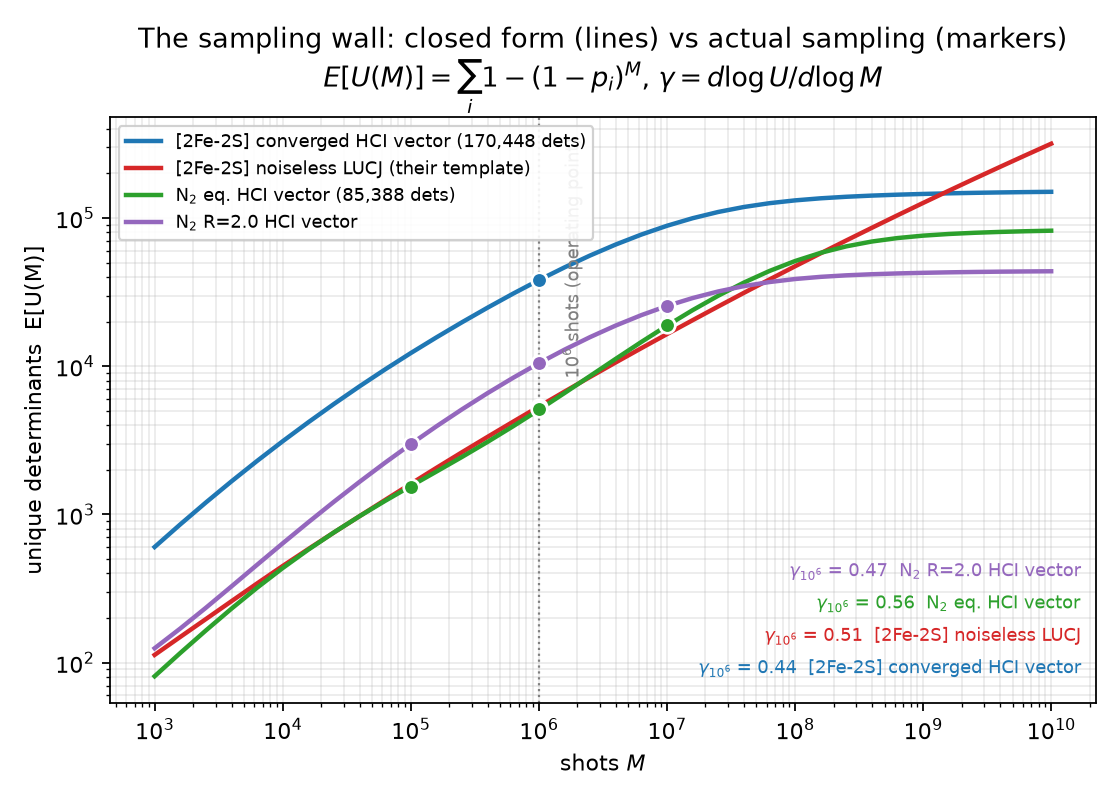
\includegraphics[width=0.8\textwidth]{fig_coupon.png}
\caption{The sampling wall as a validated law: the closed form $\mathrm{E}[U(M)]=\sum_i 1-(1-p_i)^M$ (lines) against actually-sampled unique counts (markers) for the measured distributions of this study; $\gamma = d\log U/d\log M$ annotated at the $10^6$-shot operating point.}
\label{fig:coupon}
\end{figure}

\textbf{Verdict for Layer 1:} at matched diagonalized dimension we find no regime (equilibrium, strongly correlated, or diradical, where quantum-circuit samples beat classical selected-CI. This confirms and extends arXiv:2501.07231. We emphasize the ceiling this establishes, and its exact scope: for a given prepared state, the exact-distribution arm is the \emph{noiseless, device-independent sampling limit}; no quantum computer sampling a fixed prepared state in the computational basis (the operation QSCI defines) can sample its way past its own $|c|^2$ distribution, and that limit loses at matched $D$. The bound is over \emph{samplings of a fixed state}, not over the \emph{choice} of state: a deliberately different fixed preparation (flatter amplitudes, up-weighted recoupling determinants) is a separate lever (untested here, claimed neither way), as are adaptive preparations, measurement-basis changes, and amplitude-estimation schemes, all of which lie outside this protocol and outside this claim.

\textbf{The accuracy ordering does not depend on pricing the samples.} One could object that ``matched $D$'' is a choice of cost model. It is not load-bearing: (a) the dominant cost of SQD is the classical eigensolver call (IBM's own package documentation states this, and solve cost is monotone in $D$; (b) at every matched $D$ measured here, sampled subspaces are less accurate than selected ones (the $+1.1$ to $+1.2$~mHa gaps above, at any shot price including zero); (c) where sampling does converge toward the classical curve (N$_2$), the determinant count needed for matched \emph{accuracy} is parity at best (measured inflation $0.86$--$1.38\times$, with sub-parity values arising only when the sampler draws from the classical solver's own converged vector (the proxy artifact); and (d) the shot bill is strictly additive on top. No relative pricing of shots versus CPU changes the accuracy ordering at matched $D$. (Full wall-clock at fixed $D$ additionally depends on subspace structure and solver implementation: the successor work's half-string tensor-product spaces, for instance, admit specialized Hamiltonian kernels; the claim here is the accuracy ordering at matched dimension, not total wall time.)

\subsection{The retraction: an apparent quantum win was a spin-sector artifact}\label{sec:retraction}

Round-one results at the diazene rotation TS appeared to refute the blanket ``no winning regime'': every classically-seeded arm (CIPSI and HCI from HF; HCI from CISD) stalled at $+21$--$23$~mHa even at $D=4096$ (9\% of the full sector), while exact-distribution sampling descended smoothly to $+1.9$~mHa at the same $D$. We initially attributed this to \emph{selection hysteresis}: selected CI grows around its current eigenvector and cannot tunnel to a different one at a near-degeneracy.

The spin audit shows the hysteresis is real but the scoreboard was wrong. At this geometry the lowest $M_s=0$ roots are a near-degenerate singlet/triplet pair; the classically-grown spaces were converging the \emph{triplet} while being scored against the singlet reference. Scored spin-consistently (each arm against the eigenstate it actually follows, or all arms constrained to the singlet), classical selection wins at every matched $D$ (CIPSI $+0.71$ vs sampling $+1.93$~mHa at 4096). The same audit retroactively invalidated a mechanism claim in an adjacent project of ours (a ``correlation flips the mechanism'' result that rested on the contaminated root), which we also retracted.

Two lessons carried forward. First, methodological: every stationary point in this literature needs a spin characterization before its energy has state-specific meaning. Second, adversarial: the diradical was the \emph{strongest known candidate} for a quantum-sampling win, and it died under spin resolution, so before trusting any flagship claim, the same instrument must be pointed at the flagship systems.

\subsection{The instrument: rotation-invariant \texorpdfstring{\ssq}{<S2>} for selected-CI manifolds}\label{sec:instrument}

For determinant spaces in the $M_s=0$ sector, $S^2 = S^-S^+ + S_z(S_z+1)$ reduces the spin measurement to the Gram matrix $G_{ij} = \langle S^+ v_i \,|\, S^+ v_j\rangle = \langle v_i | S^2 | v_j \rangle$ over any set of eigenvectors $\{v_i\}$. Two properties make this the right instrument for this audit:
\begin{enumerate}
\item \textbf{It is exact in the selected space}: no RDM approximations; a sparse application of $S^+$ followed by a Gram accumulation (cost: one pass over determinant pairs connected by single spin-flips).
\item \textbf{It is rotation-invariant over quasi-degenerate manifolds.} Where eigenvalues are (near-)degenerate, individual eigenvector \ssq{} values are gauge-dependent: a solver returns an arbitrary rotation within the manifold. The \emph{eigenvalues of the $S^2$ block} within the degenerate cluster are invariant, and answer the question that matters for a singlet-target mitigation claim: does the manifold \emph{contain} a singlet direction at all? (For a singlet, $S^2$ is positive semidefinite, so a zero expectation forces a zero state: a mean of 0 \emph{is} purity; for higher spin a matching \ssq{} expectation is not sufficient, and the $\langle S^4\rangle$ audit introduced below tests whether the variance vanishes.) The clustering convention (roots cluster when consecutive gaps $< 2\,\mu$Ha; Methods) is measured not to be load-bearing: re-deriving every partition in this paper at 0.2, 2, and 20~$\mu$Ha and under a residual-adaptive criterion changes none of the paper's reported clusters or block spectra (Methods, threshold scan; \texttt{\_thrscan.py}).
\end{enumerate}
Throughout this paper a scalar \ssq{} is used only for what it can support: it bounds but does not determine the spin decomposition (many weight sets share one expectation), so our claims are incompatibility statements (a singlet has $\ssq = 0$), with Gram spectra reported where manifold resolution matters. Spin, in turn, is only the \emph{first} axis of state identity: even a spin-pure root can be the wrong root of its sector, so spin moments are a necessary certificate rather than a complete one, and the full battery (spatial symmetry, particle number, overlap or root continuity against a declared target) is specified in the Recommendations.

We validated the instrument against PySCF spin labels on diazene (Gram diagonal $2.000000$, $0.000000$, $0.000000$ for a triplet/singlet/singlet triple; off-diagonals $<4\times10^{-12}$) and gate every production run on this check. (The gate is not decorative: it caught a uint64 sign-wrap defect in an earlier revision of our own code before any contaminated number was recorded.)

\subsection{[2Fe-2S]: both seeds converge to the same spin-contaminated attractor}\label{sec:fe2s2}

We audited the public Li--Chan [2Fe-2S] active space (30e,\,20o; $M_s=0$ sector dimension $2.4\times10^8$; near-exact singlet reference $E=-116.6056091$~Ha), growing determinant spaces by HCI ladders under the two seeding philosophies the controversy itself uses: a broken-symmetry (BS) two-determinant seed (the ``good guess'') and a closed-shell aufbau seed (the ``bad guess''). The followed sector-root \ssq{} and energies (Fig.~\ref{fig:s2}, Fig.~\ref{fig:err}, Table~\ref{tab:fe2s2}):

\begin{table}[ht]\centering\small
\caption{[2Fe-2S] followed sector-root energies and spin content vs subspace size $D$.}
\label{tab:fe2s2}
\begin{tabular}{lrrrrr}
\toprule
Seed & $D$ & $E_0$ (Ha) & err (mHa) & \ssq{} root0 & \ssq{} root1 \\
\midrule
BS & 1{,}011 & $-116.456202$ & $+149.4$ & 4.978 & 4.977 \\
BS & 25{,}734 & $-116.569067$ & $+36.5$ & 4.893 & 4.921 \\
BS & 65{,}124 & $-116.584165$ & $+21.4$ & 4.779 & 4.863 \\
BS & 155{,}030 & $-116.592307$ & $\mathbf{+13.3}$ & \textbf{4.659} & 4.809 \\
\midrule
aufbau & 1{,}003 & $-116.060455$ & $+545.2$ & 3.033 & 3.015 \\
aufbau & 5{,}053 & $-116.155646$ & $+450.0$ & 2.050 & 2.073 \\
aufbau & 24{,}570 & $-116.430693$ & $+174.9$ & 4.672 & 4.461 \\
aufbau & 68{,}825 & $-116.579203$ & $+26.4$ & 4.824 & 4.876 \\
aufbau & 170{,}448 & $-116.591986$ & $\mathbf{+13.6}$ & \textbf{4.669} & 4.810 \\
\bottomrule
\end{tabular}
\end{table}

Three observations.

\textbf{(i) The followed state is never a spin eigenstate.} $\ssq \approx 4.7$--$5.0$ sits between $S=1$ ($S^2=2$) and $S=2$ ($S^2=6$): a \emph{mixture}, colloquially, spin soup, not a contaminated singlet and not a clean high-spin state. The BS seed starts at exactly $S^2=5.000$ (as constructed) and decays glacially; the aufbau seed \emph{wanders} ($3.0 \to 2.05 \to 4.7$) before climbing into the same mixture band. Root~1 is equally impure ($4.8$--$4.9$ throughout): the low spectrum is spin-impure wall to wall.

\textbf{(ii) ``Good guess'' and ``bad guess'' converge to the same attractor.} By $D\approx1.6\times10^5$ the two seeds, grown under the HCI protocols audited here, agree to 0.3~mHa in energy and 0.01 in \ssq. The controversy's framing (convergence quality as a function of initial guess) dissolves at scale: selection dynamics, not the seed, controls what is being converged, and what is being converged is the compactness-favored spin mixture, not the physical singlet. The decay of \ssq{} toward the singlet value 0, normalized per doubling of $D$, is roughly constant once each arm is in the attractor (BS arm $0.085$--$0.097$ per doubling over its final three intervals; deep aufbau arm $0.106$--$0.133$), with no sign of acceleration. We stress the logical form of this observation: it is a reductio, not a forecast. Even at the fastest measured rate, reaching $\ssq < 1$ would take ${\sim}28$ further doublings, a dimension ($\approx 3\times10^{13}$) five orders of magnitude beyond the entire $2.4\times10^8$ sector, so the measured decay cannot deliver a singlet before the subspace exhausts the sector itself. The exact singlet is necessarily recovered at the full sector; what the data show is that no approach to it is visible anywhere in the observed range, and that the recovery is confined to a terminal regime about which the measured trend says nothing ($1.55\times10^5$ determinants is already 0.065\% of the sector).

\textbf{(iii) The residual error equals the physics being claimed.} Both seeds stall $+13$~mHa above the exact singlet, and the entire Heisenberg exchange ladder of [2Fe-2S] (the singlet--triplet--$\cdots$ splittings that define its magnetochemistry) spans ${\sim}15$--$30$~mHa. An unidentified-spin state with an error the size of the ladder cannot resolve the ladder. This is the precise sense in which state identity is load-bearing: at these system sizes the \emph{interesting chemistry} and the \emph{spin-identity error} live at the same energy scale.

The mechanism is the known high-spin compactness bias of truncated CI: high-spin components are representable with fewer determinants, so incremental selection over-rewards them, but its magnitude and persistence to $1.7\times10^5$ determinants on the flagship benchmark systems has not previously been measured.

\subsection{[4Fe-4S]: growth drifts away from the singlet}\label{sec:fe4s4}

The same audit on the public [4Fe-4S] active space (54e,\,36o; sector dimension ${\sim}8.8\times10^{15}$; approximate DMRG reference $-327.2396369$~Ha) gives, to our knowledge, the first spin resolution of selected-CI states on this system (Table~\ref{tab:fe4s4}).

\begin{table}[ht]\centering\small
\caption{[4Fe-4S] followed sector-root energies and spin content vs subspace size $D$.}
\label{tab:fe4s4}
\begin{tabular}{rrrrr}
\toprule
$D$ & $E_0$ (Ha) & err (mHa) & \ssq{} root0 & \ssq{} root1 \\
\midrule
1{,}106 & $-326.184317$ & $+1055.3$ & 5.293 & 5.270 \\
5{,}905 & $-326.385018$ & $+854.6$ & 6.053 & 5.914 \\
17{,}993 & $-326.445889$ & $+793.7$ & 6.464 & 6.302 \\
40{,}435 & $-326.484822$ & $+754.8$ & \textbf{7.004} & 9.284 \\
\bottomrule
\end{tabular}
\end{table}

Here \ssq{} \textbf{increases} with subspace size: from a closed-shell seed ($S^2=0$), growth monotonically \emph{recedes} from the singlet, reaching $S^2=7.0$ (past pure $S=2$) at $4\times10^4$ determinants. The low spectrum is a dense multi-spin manifold: at $D=40$k, root~1 has $S^2=9.28$ and root~2 has $S^2=5.84$; adjacent roots differ by $\Delta S^2\approx3.4$. The energies are far from the reference (probe regime; $4\times10^4$ determinants is $5\times10^{-12}$ of the sector), and we emphasize the \emph{trend}, not the endpoint: on the system where flagship SQD operates at sector fractions of ${\sim}10^{-8}$, the selection dynamics push away from the named target state, and there is no measured basis to expect singlet identity there without explicit spin control.

\subsection{The mitigation permits spin symmetry but does not produce it}\label{sec:mitigation}

Flagship SQD work addresses spin using configuration recovery plus \emph{spin-inversion closure} (the literature's ``spin completion''): augmenting the subspace with spin-inverted determinants (in the shipped software, symmetrizing the $\alpha/\beta$ half-string sets, which squares to the full spin-inverted closure of the product space). This makes the subspace invariant under spin inversion, removing an obvious obstruction to representing spin-parity eigenvectors, but it neither makes the subspace $S^2$-invariant nor guarantees that any low-energy eigenstate is a spin eigenstate. Whether the \emph{variational ground manifold within that subspace} then contains a singlet is the question our Gram instrument answers, and we tested it two ways.

\textbf{Direct audit.} At every checkpoint of every arm above (through 319{,}189 completed determinants on [2Fe-2S] and 80{,}755 on [4Fe-4S]), we spin-completed the space and re-solved. Three invariant facts, at every scale, on both systems: (a) the ground energy changes by less than $1\,\mu$Ha while the determinant count roughly doubles; (b) the ground state becomes an exactly degenerate pair $\{v,\bar v\}$ (the state and its spin-image); (c) the eigenvalues of the $2\times2$ $S^2$ block over that pair are $[x,x]$ with $x$ = the original mixture value (the $S^2$ block is proportional to the identity. Point (c) is decisive and gauge-proof: since the block is $\propto\mathbb{1}$, \emph{every} rotation within the mitigated ground manifold has the same mixed \ssq. There is no singlet in there to find. The mitigation makes spin purity \emph{permitted}; the variational principle, driven by compactness bias, declines the invitation. (A self-contained $\sim$35-second reproducer, \texttt{spin\_inversion\_is\_not\_singlet.py}, ships in the supplementary archive: on IBM's public MO FCIDUMP, the top-$N$ marginal-ranked $\alpha$ and $\beta$ half-string sets are \emph{identical}, verified at every $N$ used in this paper, including the flagship 7{,}500, so the product construction satisfies spin-inversion closure by construction, yet its ground state is strongly contaminated, $\langle S^2\rangle = 3.50$ at $N=60$; their own \texttt{solve\_fermion}/\texttt{spin\_square} agrees with our Gram instrument on that state to $1\times10^{-4}$ and 0.4~$\mu$Ha.)

\textbf{The mechanism, measured per checkpoint.} Exact pair degeneracy is not an automatic consequence of spin-inversion symmetry: symmetry alone would permit the ground to hybridize into energy-split symmetric/antisymmetric combinations across the original support and its image. Table~\ref{tab:mech} re-solves all 14 completion checkpoints of the three arms and reports the quantities that decide the mechanism: the ground-energy shift $|\Delta E_0|$ under completion; the splitting of the completed ground pair; the invariant spectrum $\{p_1, p_2\}$ of the original-support projector compressed over that pair ($p_1 = 1$ with $p_2$ small means the pair is spanned by one state on the original support and one essentially on its spin image; $p_2$ is exactly 0 for [4Fe-4S], where the two supports are disjoint, and at most 0.11 for [2Fe-2S], where they share the spin-self-inverse determinants on which the image member retains a little projector weight); the Hamiltonian coupling $\|P_+ H v\|$ from the uncompleted ground $v$ to the added determinants; and the invariant $S^2$ block. The pattern is uniform. The added spin-image support is $H$-uncoupled from the converged ground at the solve's own residual scale ($\|P_+ H v\| \le 2.5\times10^{-9}$~Ha), so the ground persists identically: $|\Delta E_0| \le 8\times10^{-13}$~Ha, with the localized pair member carrying ${<}\,10^{-14}$ of its weight on the added determinants, and its spin image enters as the second member of an exactly degenerate pair (splitting $\le 1.9\times10^{-12}$~Ha against a solver tolerance of $10^{-9}$) rather than hybridizing into split combinations. The measured coupling is the quantitative content of ``permits but does not produce'': completion adds the support that spin symmetry needs, but the variational state it was meant to repair is dynamically disconnected from that support.

\begin{table}[t]
\centering
\caption{Completion-mechanism audit at every spin-completion checkpoint (Section 2.6): energy shift under completion, completed-pair splitting, invariant original-support projector spectrum $\{p_1,p_2\}$ over the ground pair, coupling from the uncompleted ground to the added determinants, and the invariant $S^2$ block of the pair. $^\dagger$Dense-adjudicated row: the iterative solver returned one member per degenerate pair on this space (splitting reported by the dense solve). Data: \texttt{degen.npz}, \texttt{degen\_dense.npz}.}
\label{tab:mech}
\small
\setlength{\tabcolsep}{4pt}
\resizebox{\textwidth}{!}{\begin{tabular}{llccccc}
\hline
space & $D \to D'$ & $|\Delta E_0|$ (Ha) & pair split (Ha) & $p_1$, $p_2$ & $\|P_+ H v\|$ (Ha) & $S^2$ block \\
\hline
{[2Fe-2S]} BS & 1,011 $\to$ 2,020 & $2.8\times10^{-13}$ & $2.8\times10^{-13}$ & 1.0000, 0.0168 & $5.7\times10^{-10}$ & [4.9783, 4.9783] \\
{[2Fe-2S]} BS & 5,574 $\to$ 11,146 & $5.7\times10^{-14}$ & $2.6\times10^{-13}$ & 1.0000, 0.0645 & $3.2\times10^{-10}$ & [4.9778, 4.9778] \\
{[2Fe-2S]} BS & 25,734 $\to$ 51,466 & $7.1\times10^{-14}$ & $1.3\times10^{-13}$ & 1.0000, 0.0510 & $4.5\times10^{-11}$ & [4.8934, 4.8934] \\
{[2Fe-2S]} BS & 65,124 $\to$ 130,246 & $4.3\times10^{-14}$ & $2.7\times10^{-13}$ & 1.0000, 0.0441 & $6.1\times10^{-11}$ & [4.7792, 4.7792] \\
{[2Fe-2S]} BS & 116,270 $\to$ 232,538 & $2.4\times10^{-13}$ & $5.1\times10^{-13}$ & 1.0000, 0.0411 & $9.9\times10^{-12}$ & [4.6978, 4.6978] \\
{[2Fe-2S]} BS & 155,030 $\to$ 310,058 & $4.3\times10^{-13}$ & $4.3\times10^{-13}$ & 1.0000, 0.0398 & $2.0\times10^{-11}$ & [4.6592, 4.6592] \\
{[2Fe-2S]} aufbau & 33,632 $\to$ 45,557 & $2.0\times10^{-13}$ & $3.8\times10^{-13}$ & 1.0000, 0.1085 & $9.7\times10^{-10}$ & [4.9545, 4.9545] \\
{[2Fe-2S]} aufbau & 71,412 $\to$ 121,117 & $3.0\times10^{-13}$ & $3.4\times10^{-13}$ & 1.0000, 0.0511 & $2.5\times10^{-9}$ & [4.8095, 4.8095] \\
{[2Fe-2S]} aufbau & 109,151 $\to$ 196,595 & $7.4\times10^{-13}$ & $5.0\times10^{-13}$ & 1.0000, 0.0476 & $6.4\times10^{-10}$ & [4.7452, 4.7452] \\
{[2Fe-2S]} aufbau & 170,448 $\to$ 319,189 & $9.9\times10^{-14}$ & $1.4\times10^{-14}$ & 1.0000, 0.0460 & $7.5\times10^{-10}$ & [4.6688, 4.6688] \\
{[4Fe-4S]} & 1,106 $\to$ 2,097$^\dagger$ & $5.7\times10^{-14}$ & $0$ & 1.0000, 0.0000 & $3.1\times10^{-16}$ & [5.2930, 5.2930] \\
{[4Fe-4S]} & 5,905 $\to$ 11,695 & $3.4\times10^{-13}$ & $1.7\times10^{-13}$ & 1.0000, 0.0000 & $1.7\times10^{-10}$ & [6.0527, 6.0527] \\
{[4Fe-4S]} & 17,993 $\to$ 35,871 & $8.0\times10^{-13}$ & $1.9\times10^{-12}$ & 1.0000, 0.0000 & $1.5\times10^{-10}$ & [6.4644, 6.4644] \\
{[4Fe-4S]} & 40,435 $\to$ 80,755 & $5.7\times10^{-14}$ & $2.3\times10^{-13}$ & 1.0000, 0.0000 & $2.9\times10^{-10}$ & [7.0044, 7.0044] \\
\hline
\end{tabular}}
\end{table}

One checkpoint required adjudication ($\dagger$). At the coarsest [4Fe-4S] space ($1{,}106 \to 2{,}097$ determinants) the iterative Davidson solver used throughout this audit returned only one member of each degenerate pair: a unique-looking completed ground with a spurious 93~mHa ``gap'' to a state that is in fact the next pair's lower member. Dense diagonalization of the full 2,097-dimensional block restores the exact structure (ground-pair splitting 0 to machine precision, $\{p_1, p_2\} = \{1.000000, 0.000000\}$, $S^2$ block $[5.2930, 5.2930]$), the same mechanism in its cleanest realization, and confirms the asymmetric-space energy and \ssq{} records to all stored digits. We flag the adjudication rather than silently replacing the row because it is a live instance of this paper's warning: on degenerate manifolds, iterative eigensolver output is not self-certifying, and the manifold instruments must be gauged against an independent solve (\texttt{degen.npz}, \texttt{degen\_dense.npz}).

\textbf{As-shipped audit.} To foreclose ``you reimplemented our mitigation incorrectly,'' we ran IBM's \texttt{qiskit-addon-sqd} pipeline exactly as shipped (its \texttt{diagonalize\_fermionic\_hamiltonian} driver, its post-selection, its configuration-recovery loop, its Cartesian-product subspace construction, its \texttt{symmetrize\_spin} option, and its own \texttt{SCIState.spin\_square()} diagnostic) on $10^6$ samples drawn from our converged [2Fe-2S] vector ($D=170{,}448$, $\ssq=4.669$; the kind of state a benchmark following this protocol actually produces). Results (batch means over 3 batches, \texttt{samples\_per\_batch}=500, 4 recovery iterations), Table~\ref{tab:asshipped}:

\begin{table}[ht]\centering\small
\caption{As-shipped \texttt{qiskit-addon-sqd} on $10^6$ soup-vector samples (batch means; \texttt{symmetrize\_spin=True}).}
\label{tab:asshipped}
\begin{tabular}{crrrr}
\toprule
Iteration & subspace & $E$ (Ha) & err (mHa) & their \ssq \\
\midrule
1 & ${\sim}59{,}000$ & $-116.513$ & $+92.8$ & 4.90 \\
2 & ${\sim}114{,}000$ & $-116.542$ & $+63.3$ & 4.87 \\
3 & ${\sim}158{,}000$ & $-116.553$ & $+52.6$ & 4.85 \\
4 & ${\sim}193{,}000$ & $-116.560$ & $\mathbf{+45.7}$ & \textbf{4.837} \\
\bottomrule
\end{tabular}
\end{table}

The best single batch reaches $-116.560107$~Ha ($+45.5$~mHa) with their-$\ssq=4.834$. Three findings:
\begin{enumerate}
\item \textbf{Energy moves, spin does not.} Their own diagnostic reports $\ssq = 4.90 \to 4.84$ across four configuration-recovery iterations. Recovery optimizes energy monotonically ($+92.8 \to +45.7$~mHa) while spin identity is essentially frozen: the loop descends \emph{within} the spin-contaminated manifold.
\item \textbf{The mitigation is a measured no-op.} Running the identical experiment with \texttt{symmetrize\_spin=False}: every batch of every iteration agrees with the symmetrized run to $\Delta E < 10^{-9}$~Ha and $\Delta\ssq \sim 10^{-11}$, while the symmetrized subspace is exactly $4.00\times$ larger (194{,}481 vs 48{,}600 determinants at iteration 4). The spin-completed determinants receive zero variational weight: the permits-vs-produces mechanism of the direct audit, reproduced inside the shipped code, measured by the shipped diagnostic.
\item \textbf{Matched-dimension inversion.} The pipeline's best energy, $+45.5$~mHa at $1.9\times10^5$ determinants, is $3.3\times$ further from the exact singlet than the $+13.6$~mHa of the classical HCI space \emph{that generated the samples} at comparable size ($1.7\times10^5$). Sampling and recovering a selected-CI state is strictly worse than keeping the selected-CI state. The coupon-collector wall ($10^6$ shots $\to$ 38{,}118 unique determinants) discards most of the parent space and recovery cannot rebuild it at matched dimension.
\end{enumerate}

We note explicitly: the shipped solver (\texttt{solve\_sci}, backed by PySCF's \texttt{kernel\_fixed\_space}) accepts a \texttt{spin\_sq} argument wired to PySCF's \texttt{fix\_spin\_} spin-penalty, the mechanism intended to suppress non-singlet character directly. The shipped recovery loop leaves it at its default, \texttt{None}. Nor is the mechanism obscure to this community: the flagship's own Methods state that ``we achieve the conservation of total spin by a soft constraint in the eigenstate solver, i.e. by adding a penalty term to mitigate spin contamination,'' the squared constraint $H+\lambda[S^2-s(s+1)]^2$ employed at $\lambda=0.2$; an IBM-adjacent methylene study (arXiv:2411.04827) uses exactly this Lagrange-penalty construction in an SQD context; and a 2026 preprint applies it to this very [2Fe-2S] active space (arXiv:2603.09346, $\lambda=0.1$, whose best energy, $-116.49986$~Ha, still lands $+105.8$~mHa above the DMRG reference distributed with the flagship's own data). A mechanism aimed at the failure we measure is known, implemented, stated by the flagship as employed, and off by default in the shipped package; and wherever it appears, stated or switched on, the achieved \ssq{} goes unreported.

\textbf{The penalty, switched on.} The rebuttal this invites (\emph{run it with the penalty on}, which is also what the flagship's Methods state was done) has a measured answer, and it is not the one the switch's existence suggests. We took the shipped pipeline's own converged [2Fe-2S] subspaces (the symmetrized product spaces behind the $+45.5$~mHa row above, captured at recovery iterations 1 and 4, $D = 245^2$ and $441^2$; each space's unpenalized ground reproduces the shipped record and agrees with an independent PyCI diagonalization of the same determinants to 0.00~$\mu$Ha) and computed the ground state of $H + \lambda S^2$ (the exact linear operator PySCF's \texttt{fix\_spin\_(ss=0)} applies at $M_s = 0$) as a function of penalty strength $\lambda$, recording the true energy $\langle H\rangle$ (from the RDMs, as the shipped solver does) and both spin moments of every converged state (Table~\ref{tab:penalty}, on the operating-point $D = 441^2$ space; the $D = 245^2$ space behaves identically).

\begin{table}[ht]\centering\small
\caption{Ground state of $H + \lambda S^2$ on the shipped pipeline's own converged [2Fe-2S] soup subspace ($D = 441^2$, the $+45.5$~mHa row of Table~\ref{tab:asshipped}). $\lambda S^2$ is the exact linear penalty PySCF's \texttt{fix\_spin\_(ss=0)} applies at $M_s = 0$; energies and moments are the true $\langle H\rangle$, \ssq, and $\mathrm{Var}(S^2)$ of each converged root.}
\label{tab:penalty}
\begin{tabular}{lrrrr}
\toprule
penalty strength $\lambda$ & $E$ (Ha) & err (mHa) & \ssq & $\mathrm{Var}(S^2)$ \\
\midrule
0 (off, the $+45.5$ mHa row) & $-116.560107$ & $+45.5$ & 4.834 & 1.89 \\
0.1 (\texttt{fix\_spin\_}'s shipped default) & $-116.533031$ & $+72.6$ & 4.165 & 0.83 \\
0.2 (the flagship's stated strength, in this linear form) & $-116.494963$ & $+110.6$ & 3.902 & 0.48 \\
0.5 & $-116.341427$ & $+264.2$ & 3.441 & 0.18 \\
$\geq 1$ (singlet sector) & $-113.711$ & $\mathbf{+2895}$ & $\mathbf{0.0000}$ & $\mathbf{0.0000}$ \\
\bottomrule
\end{tabular}
\end{table}

The trade-off is a frontier with no competitive interior. Through $\lambda = 0.1$ (the shipped default) and 0.2 the penalty anneals \ssq{} only from 4.83 to 3.90 while the true energy rises monotonically from $+45.5$ to $+111$~mHa; the ground stays in the spin-contaminated band ($\ssq \geq 3.4$) out to $+264$~mHa; and the first genuine singlet, the lowest exact spin-0 eigenstate the subspace can represent ($\ssq = \mathrm{Var}(S^2) = 0.0000$, residual $10^{-8}$)), sits \textbf{2.9~Hartree above the reference} (the $D = 245^2$ space floors at $+3.03$~Ha; the lowest closed-shell determinant in either space, itself a singlet, independently lies at $+3.05$~Ha). The monotone rise is structural: $\lambda S^2$ is positive semidefinite, so within a fixed subspace the penalized ground's true energy can only exceed the unpenalized minimum, and the singlet end of the frontier is the lowest-energy exact singlet the subspace contains. No penalty strength yields a singlet at competitive energy because the sampled subspace holds none, consistent with marginal-product selection retaining the determinants energy needs while omitting the spin-recoupling partners identity needs. The spin--energy vise of Section~\ref{sec:theirsamples} is therefore not a solver choice or a tuning failure; it is the geometry of the sampled subspace, with the jaws separated by nearly three Hartree (Figure~\ref{fig:penalty}). The same positive-semidefiniteness closes the \emph{other} jaw without a further run: the low-\ssq{} hardware and template subspaces of Section~\ref{sec:theirsamples} already sit $+229$ to $+248$~mHa above the reference, and a penalty cannot lower $\langle H\rangle$ below a subspace's unpenalized minimum, so no jaw of the vise yields a competitive singlet under any spin penalty, one jaw by direct measurement and the others by the semidefiniteness of $\lambda S^2$.

\textbf{The flagship's stated form, at the flagship's stated strength.} The flagship Methods state the constraint in squared form, $H+\lambda[S^2-s(s+1)]^2$ with $\lambda=0.2$ (singlet target $s=0$, so the penalty is $\lambda(S^2)^2$). Compressing $(S^2)^2$ onto a fixed determinant subspace $P$ is not unique, and the ambiguity is this paper's own subject: a Krylov eigensolver confined to $P$ applies the \emph{projected square} $(PS^2P)^2$, the projected operator squared inside the subspace, whereas the literal matrix compression of $(S^2)^2$ is $P(S^2)^2P$, which lets $S^2$ leave $P$ and return. The two differ by the positive-semidefinite leakage operator $P(S^2)^2P - (PS^2P)^2 = PS^2(I-P)S^2P \succeq 0$, whose non-vanishing \emph{is} the noncommutation $[PHP,\, PS^2P] \neq 0$ at the center of this work; it cannot be assumed negligible, so we built both operators (the literal square via the exact $M_s=0$ spin ladder, the $S^+$ machinery of the second-moment kernel, gauged operator-for-operator against PySCF's independent $S^2$ to machine precision) and ran each on the benchmark-energy subspace at the stated $\lambda=0.2$ (\texttt{\_sqdpen\_true.py}, \texttt{sqdpen\_true\_it4.npz}; \texttt{\_sqdpen\_sq.py}, \texttt{sqdpen\_sq\_it4.npz}, each $\lambda=0$ anchor reproducing the shipped record under the same gates). The two compressions bracket the outcome, and neither is a competitive singlet. The \textbf{projected square} lands the ground at $+528$~mHa with $\ssq = 3.010$, an 11.6-fold increase over the unpenalized error and still three units of \ssq{} from the singlet, and it sharpens the mechanism into its cleanest exhibit: the converged state is nearly an eigenvector of the \emph{projected} operator $PS^2P$, in-subspace variance 0.009 concentrated at 3.01, which is not $S(S+1)$ for any $S$, while its exact first moment alone forces a physical spin variance of at least $(\ssq-2)(6-\ssq) \approx 3.0$, because the physical $S^2$ spectrum is the lattice $\{0, 2, 6, 12, \ldots\}$ and the minimum-variance distribution at a fixed mean lives on the two adjacent points. Certainty in the wrong operator: sharp in $PS^2P$ at an unphysical spin value, broad in $S^2$ itself. The \textbf{literal square} $P(S^2)^2P$, carrying the leakage the projected form drops, is the stronger penalty: it registers the unpenalized state's full $\langle S^4\rangle \approx 47$, not its in-subspace proxy $\approx 23$, and at the same stated $\lambda=0.2$ it drives the ground past a sharp threshold to a singlet at the subspace's floor: $\ssq = 0.004$, $\mathrm{Var}(S^2) = 0.03$, at $+2{,}884$~mHa (the $D=245^2$ space reaches $\ssq = 0.000$ at $+3{,}034$~mHa; the sweep resolves the transition, the literal square holding $\ssq \approx 3.0$ with broad physical variance $\approx 9$ through $\lambda=0.1$, then snapping to the floor by $\lambda=0.2$). The projected square cannot leave the contaminated band; the literal square reaches a singlet only by paying the subspace's full $+2.9$~Ha floor. That the two endpoints coincide with the linear frontier's floor is guaranteed, not fitted: $(S^2)^2$, $(PS^2P)^2$, and $S^2$ are all positive semidefinite with the identical null space, the exact singlets ($PS^2P\,c=0 \iff \langle c|S^2|c\rangle=0 \iff S^2 c=0$), so every penalty of this family shares the same $+2.9$~Ha floor in any compression, and positive-semidefiniteness holds each above the subspace's unpenalized minimum. This is the Discussion's noncommutation made operational: the penalty pulls the ground toward eigenvectors of the spin operator, the energy toward eigenvectors of $PHP$, and on a subspace where the two do not commute the compromise carries neither identity, whether the penalty is realized as the projected square, pinned at the wrong value, or the literal square, driven to a singlet 2.9~Ha too high.

Two corollaries complete the rebuttal. First, the shipped penalty path does not even reach this frontier: PySCF's \texttt{fix\_spin\_} as \texttt{solve\_sci} wires it returns \texttt{converged = False} on all five (space, shift, \texttt{max\_cycle}) arms we ran (both shifts, at the silent default \texttt{max\_cycle} and at \texttt{max\_cycle = 600}), each landing 0.27--0.33~Ha above the penalized minimum we certify (Figure~\ref{fig:penalty}, panel B). Handed our converged penalized ground state as its initial guess, however, the same kernel confirms it: \texttt{converged = True}, overlap 1.000000, penalized Rayleigh quotient equal to ours to machine precision, so the cold-start failure is an initial-guess pathology, not a disagreement about the minimum, and the certification of the frontier is their own code's. The one mitigation the tooling advertises as spin-targeting fails silently when it is switched on. Second, running the \emph{entire} configuration-recovery protocol end to end with the penalty active ($ss = 0$, converged solves) reproduces the frontier rather than escaping it: at $\lambda = 0.2$ the full loop returns $+110.4$~mHa at $\ssq = 3.93$, and at $\lambda = 0.1$, $+72.6$~mHa at $\ssq = 4.18$; both match the fixed-space frontier to tenths of a mHa, both are worse in energy than the unpenalized $+45.5$~mHa, and neither is closer to a singlet. The penalty-matched rerun of the published protocol lands exactly where the subspace geometry says it must.

\begin{figure}[ht]\centering
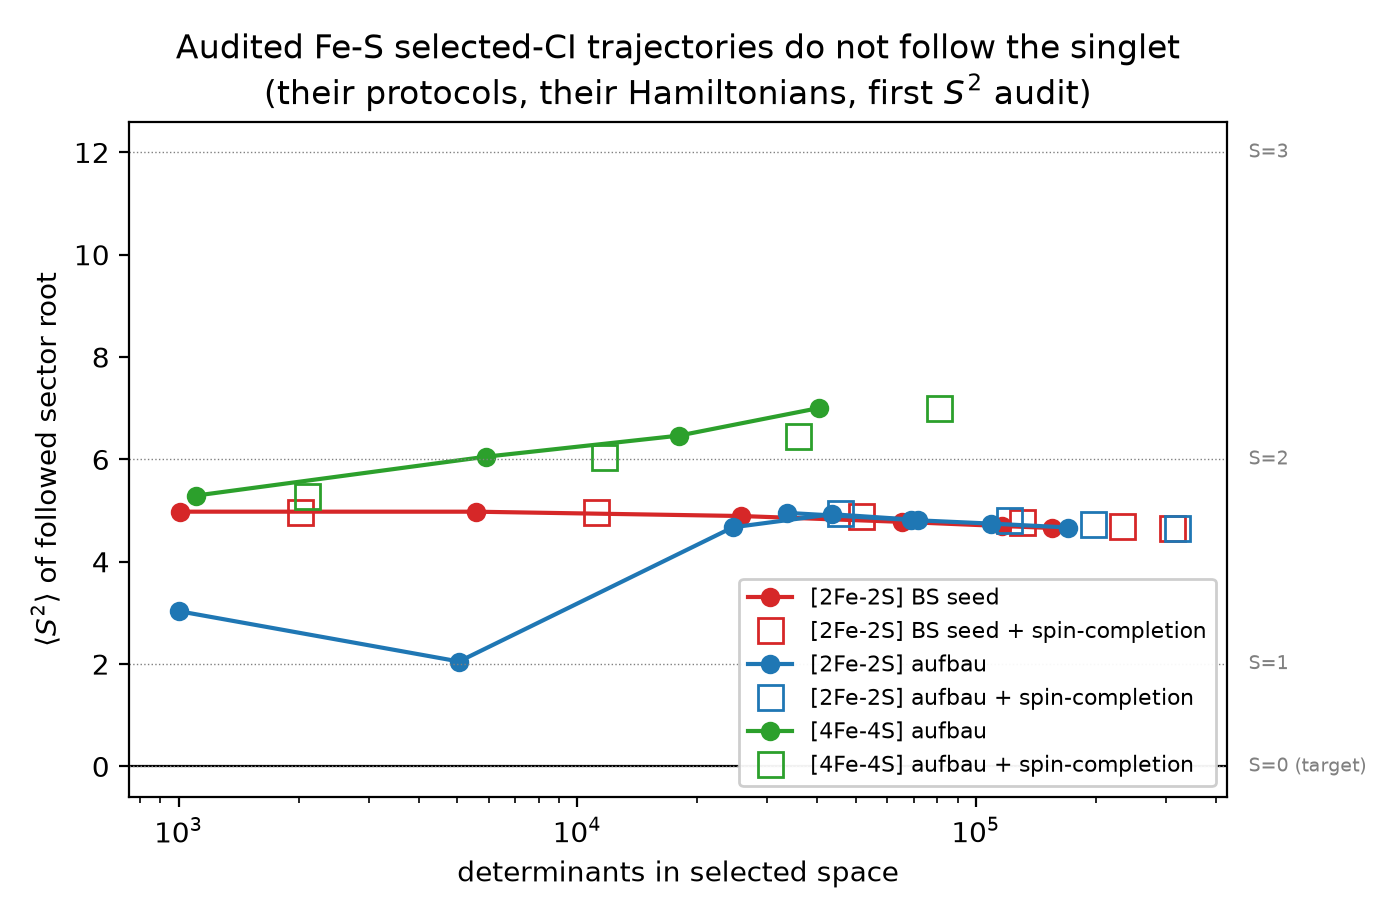
\includegraphics[width=0.85\textwidth]{fig_s2_vs_d.png}
\caption{\ssq{} of the followed sector root vs subspace size for all audit arms. Open squares: the spin-completed (mitigated) spaces, identical to the unmitigated points. Dotted rails: pure spin eigenvalues.}
\label{fig:s2}
\end{figure}

\begin{figure}[ht]\centering
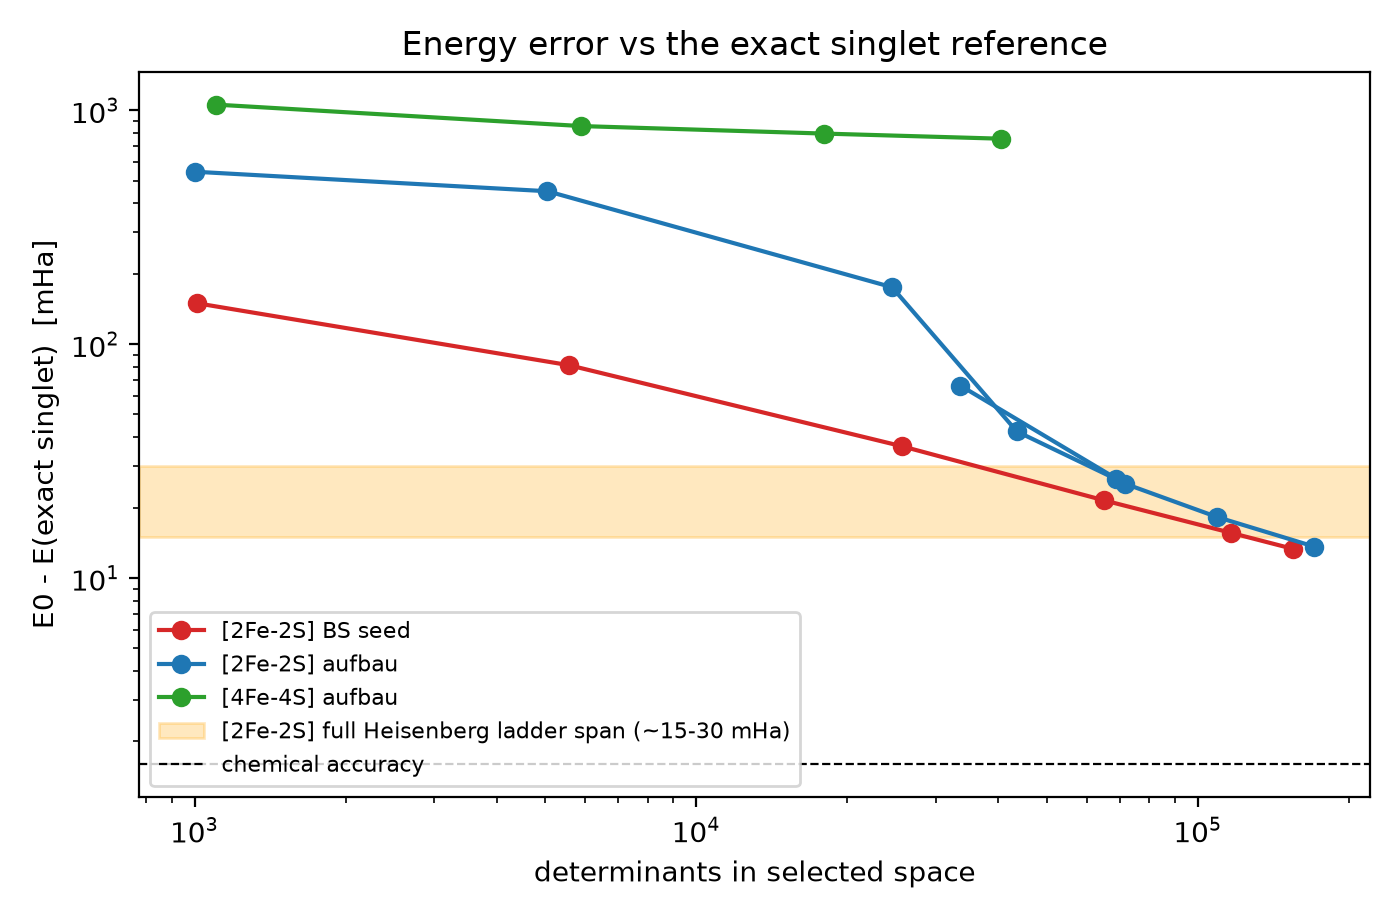
\includegraphics[width=0.85\textwidth]{fig_err_vs_d.png}
\caption{Energy error vs the exact singlet reference. Shaded band: the [2Fe-2S] Heisenberg-ladder span (${\sim}15$--$30$~mHa); dashed line: chemical accuracy.}
\label{fig:err}
\end{figure}

\begin{figure}[ht]\centering
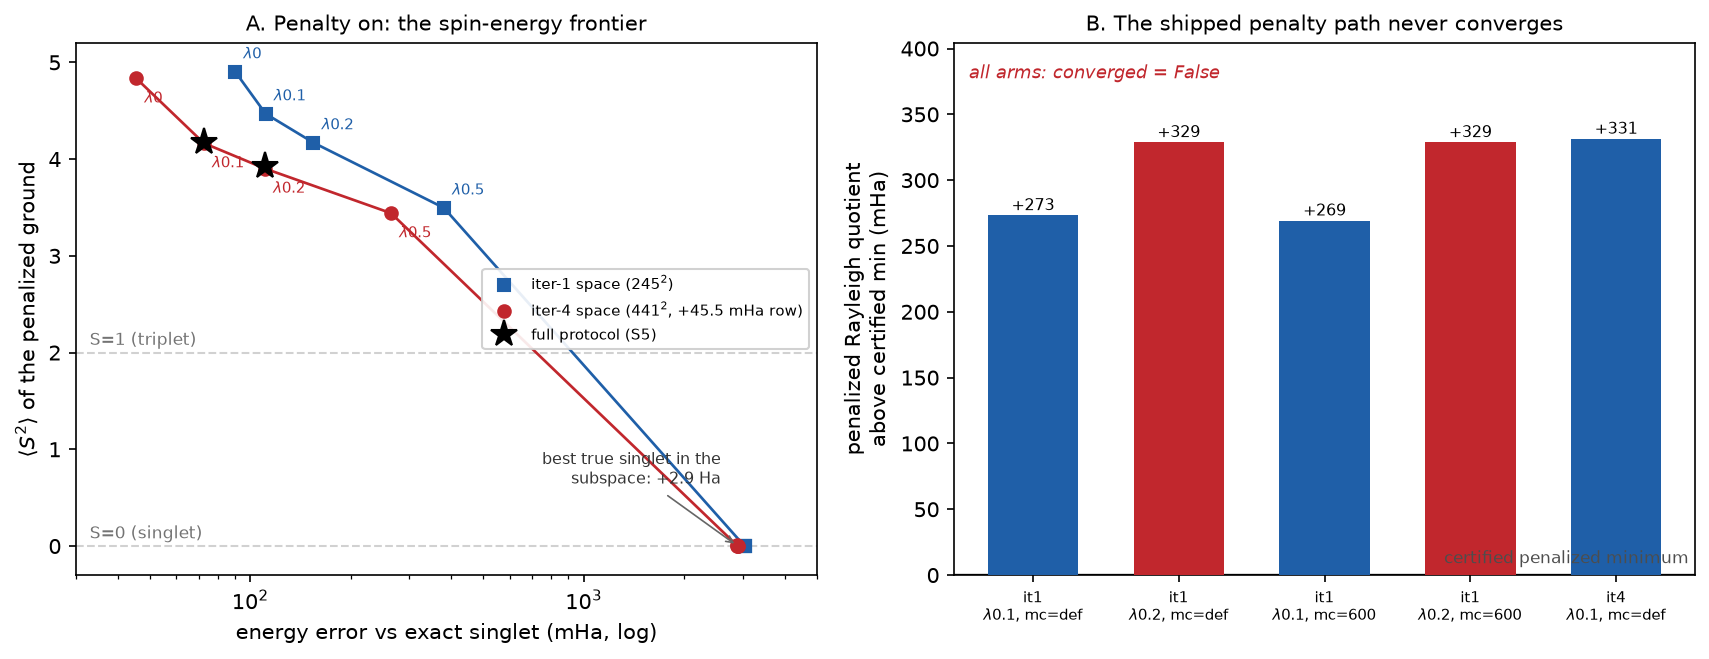
\includegraphics[width=\textwidth]{fig_penalty_frontier.png}
\caption{Penalty on, on the shipped pipeline's own [2Fe-2S] soup subspaces. \textbf{A}: the spin--energy frontier, \ssq{} of the ground of $H + \lambda S^2$ vs its true energy error, for the captured $D = 245^2$ (iter-1) and $D = 441^2$ (iter-4, the $+45.5$~mHa row) subspaces, markers at each $\lambda$, spin-ladder rails at $S(S+1) = 0, 2$; the full penalized recovery protocol overlaid as stars. The jaws (benchmark energy at $\ssq \approx 4.8$, a genuine singlet at $+2.9$~Ha) are $\sim$3~Hartree apart, with nothing competitive between. \textbf{B}: the shipped penalty path never converges; each \texttt{kernel\_fixed\_space} $+$ \texttt{fix\_spin\_(ss=0)} arm returns \texttt{converged=False}, 0.27--0.33~Ha above the certified penalized minimum.}
\label{fig:penalty}
\end{figure}

\subsection{IBM's own data archive: the flagship samples were public all along}\label{sec:archive}

The Science Advances data-availability statement points to a public repository (\url{https://github.com/jrm874/sqd_data_repository}, archived as DOI \href{https://doi.org/10.5281/zenodo.15324153}{10.5281/zenodo.15324153}) that turns out to contain far more than integrals: the \textbf{raw hardware measurement outcomes} of the flagship experiments ([2Fe-2S]: 2{,}457{,}600 shots from December 2023, as 300 batches of 8{,}192; [4Fe-4S]: 3{,}163{,}742 recorded outcomes from April 2024, with device job IDs), the MO-basis FCIDUMPs those experiments used, the LUCJ circuit-generation template, a variationally \emph{optimized} [2Fe-2S] LUCJ circuit together with \textbf{58{,}644{,}964 noiseless samples drawn from it}, SQD-on-uniform-random null controls, classical HCI ladders, and a configuration-recovery ablation study. Everything in this section derives from that archive processed by the as-shipped \texttt{qiskit-addon-sqd}: their samples, their Hamiltonians, their pipeline, their spin diagnostic.

\textbf{One spectrum, two bases.} Their [2Fe-2S] FCIDUMP is in canonical RHF orbitals: the identity-basis aufbau determinant reproduces their tabulated RHF energy ($-116.205816$~Ha) exactly (largest off-diagonal Fock element $4\times10^{-7}$), and their tabulated DMRG reference, $-116.6056091$~Ha, is \emph{identical} to the near-exact reference of the Li--Chan-basis dumps used in Sections~\ref{sec:fe2s2}--\ref{sec:mitigation}, the same active space under a unitary orbital rotation, certifying that our audits and their experiments address one and the same spectrum.

\textbf{Their own null control: uniform random bitstrings match their [2Fe-2S] hardware.} The archive's \texttt{sqd\_on\_uniform\_distribution} files run their pipeline on uniform random samples. On [2Fe-2S], the flagship system small enough for uniform sampling to compete: the uniform control \textbf{matches or beats the hardware samples in every published comparison}. The three published eigenstate files contain two independent evidence streams, a structure we verified row-by-row before counting anything (and which the audit script asserts): the eigenstate-B hardware file is a strict subset of C's (all 59 of B's rows appear bit-identically in C, which carries 7 more) and the B and C uniform files are byte-identical, so B/C constitutes a single stream; eigenstate A shares no rows with either, and its energies differ from C's at common dimensions. Best energies (hardware minus uniform): $+1.90$~mHa (stream A, with the uniform run using \emph{smaller} maximum subspaces, $1.6\times10^7$ vs $5.6\times10^7$) and $+12.17$~mHa (stream B/C). Batch-resolved, this is not a best-of artifact: at all 9 (stream, dimension) conditions the two protocols share (each hardware file paired with its own uniform null, 5--10 hardware and 10 uniform batches per condition), the uniform-control \emph{mean} energy is lower than the hardware mean, by 4.8--14.9~mHa on stream A and 18.4--26.7~mHa on stream B/C, against per-group sample standard deviations of 3.7--16.3~mHa; within conditions, whose batches are disjoint shot groups, the uniform advantage is individually significant (two-sided Mann--Whitney, $p<0.05$) at 7 of the 9 (the two smallest-subspace conditions of stream A are not). We attach no global significance level across conditions: dimensions within a stream re-process the same released sample pool, so the nine conditions are repeated measures on two independent evidence streams, not nine independent experimental units; the direction (uniform mean $\le$ hardware mean) holds in all nine, in both streams. (An earlier draft counted the B and C files as separate evidence, 13 points; the row-level structure audit corrected this to 9.) All of these runs, hardware and uniform alike, sit $+140$ to $+184$~mHa above their DMRG reference at subspace dimensions up to $5.6\times10^7$. Under every released [2Fe-2S] comparison available for audit, the hardware samples yield no energy advantage over the corresponding uniform-random control.

\textbf{Headline scale, their own numbers.} For [4Fe-4S], the archive's largest published runs (100 batches at subspace dimension $d=10^8$) reach a best energy of $-326.644824$~Ha, \textbf{$+594.8$~mHa above their DMRG reference}, improving only ${\sim}53$~mHa per decade of subspace growth over $d = 9\times10^6 \to 10^8$. Their own classical HCI benchmark file reports $-326.793854$~Ha ($+445.8$~mHa): at the flagship operating point, on the flagship system, \textbf{the archive's own quantum-sampled energies trail its own classical-selection energies by ${\sim}149$~mHa}. (Hardware does beat \emph{uniform} sampling here, by ${\sim}1.06$~Ha, as it must at 36 orbitals, where uniform 72-bit strings essentially never land anywhere useful; we measure the raw hardware samples' own correct-sector rate at $5.4\times10^{-4}$ in Section~\ref{sec:rawladder}.)

\textbf{Their own ablation: the classical recovery does the work.} The archive's \texttt{N2\_6-31G\_recovery\_effect} study, run by the authors themselves, shows that with configuration recovery disabled their noiseless N$_2$ SQD errors are 1.1--1.8~\emph{Hartree}; with recovery enabled, 4--7~mHa, a three-orders-of-magnitude gap attributable entirely to the classical post-processing, at zero noise. In this ablation, the samples do not carry the accuracy; the classical machinery reconstructs it.

\subsection{Their samples through their pipeline: the audit of the experiments as released}\label{sec:theirsamples}

This section closes the two limitations a rebuttal would otherwise lead with (``not our samples''; ``not our subspace provenance''). We ran the as-shipped pipeline with identical knobs (\texttt{samples\_per\_batch}=500, 3 batches, \texttt{max\_dim}=500, seed 17) on every input class the archive makes possible, reading spin with the pipeline's own diagnostic at every iteration (Table~\ref{tab:theirsamples}; a fixed-knob comparison across input classes; the hardware leg is then extended to the flagship's own published construction and dimensions in Table~\ref{tab:rawladder}).

\begin{table}[ht]\centering\small
\caption{As-shipped pipeline on every available [2Fe-2S] input class (their MO basis where the input is theirs; identical knobs throughout).}
\label{tab:theirsamples}
\begin{tabular}{p{7.2cm}rrr}
\toprule
input & best $E$ (Ha) & err vs their DMRG (mHa) & their \ssq \\
\midrule
$10^6$ samples of the converged classical benchmark state (Sec.~\ref{sec:mitigation}, Li--Chan basis; err vs same-spectrum exact) & $-116.560107$ & $\mathbf{+45.5}$ & \textbf{4.834} \\
\textbf{their 2{,}457{,}600 raw hardware shots (the flagship experiment's own data)} & $-116.358076$ & $+247.5$ & 0.235 \\
$10^6$ noiseless samples, their circuit template (CCSD $t_1{+}t_2$, their pairs) & $-116.376680$ & $+228.9$ & 0.108 \\
uniform draws from their published 58.6M-configuration set ($2\times10^6$-entry subsample, unit counts) & $-116.103827$ & $+501.8$ & 2.008 \\
\bottomrule
\end{tabular}
\end{table}

Additions to the shipped-pipeline findings of Section~\ref{sec:mitigation}:

\textbf{The hardware leg is certified against their own energetics.} Reconstructing shot counts from their archive reproduces the documented protocol exactly (300 batches $\times$ 8{,}192 = 2{,}457{,}600 shots), and our best energies at subspace dimension $2.5\times10^5$ are consistent with their published energy--variance rows at the same dimension. We report sector rates as context for what configuration recovery must accomplish: the pipeline is designed to process out-of-sector samples, so a low rate is not a defect by itself. We measure the raw samples' correct-particle-sector rate at \textbf{0.445\%}: 99.55\% of the flagship experiment's shots lie outside the physical sector, and the reported subspaces and energies are reconstructed from this small in-sector fraction by the classical recovery loop, consistent with their recovery-ablation study (Section~\ref{sec:archive}).

\textbf{The spin--energy vise.} The first three input classes triangulate a trade-off that no run escapes: samples of a converged benchmark-protocol state reach benchmark-grade energies ($+45.5$~mHa) but are strongly spin-contaminated ($\ssq = 4.83$); their actual hardware samples and their ansatz's ideal noiseless samples return states with low scalar $\ssq = 0.11$--$0.24$ but energetically noncompetitive ($+229$ to $+248$~mHa; the coupon wall of Section~\ref{sec:nowin} caps the usable subspace); a low mean is not a clean singlet, and their nonzero variances ($\mathrm{Var}(S^2) = 0.64$--$1.36$, Section~\ref{sec:crossinst}) show these too are spin mixtures, not eigenstates. \textbf{Nothing simultaneously approaches the energy and the identity.} We also note the mitigation's only measurable energetic success lives on the wrong side of this vise: \texttt{symmetrize\_spin} changes nothing ($<1$~nHa) on spin-mixed input, but buys 7.7--9.5~mHa on the low-$\ssq$ noiseless/hardware inputs; it helps only on inputs whose returned states already have a low scalar $\ssq$ (their variances notwithstanding) and whose energy is noncompetitive.

\subsection{The raw-counts ladder at their published construction}\label{sec:rawladder}

\textbf{The hardware leg at their published construction: dimension buys energy by spending spin.} The fixed comparison knobs above answer the cross-input question; to audit the actual experiment at its own published operating points, we re-ran the identical pipeline on the same 2{,}457{,}600 raw shots at the flagship's own construction: 10 batches per dimension, 5 recovery iterations, \texttt{max\_dim} $= N \in \{500, 1000, 2000\}$ strings per spin, giving subspace dimensions $N^2 = 2.5\times10^5$, $10^6$ and $4\times10^6$ (the largest [2Fe-2S] dimension published below the HPC-scale runs); Table~\ref{tab:rawladder}.

\begin{table}[ht]\centering\small
\caption{Their raw hardware shots at their published construction (10 batches, 5 recovery iterations, \texttt{max\_dim} $=N$): the converged dimension ladder.}
\label{tab:rawladder}
\begin{tabular}{lrrrr}
\toprule
\texttt{max\_dim} $N$ (dim $N^2$) & best $E$ (Ha) & err (mHa) & their \ssq & their published best-of-10 (mHa) \\
\midrule
500 ($2.5\times10^5$) & $-116.368271$ & $+237.3$ & 0.142 & $+266.3$ \\
1000 ($10^6$) & $-116.390277$ & $+215.3$ & 0.108 & $+238.8$ \\
2000 ($4\times10^6$) & $-116.438440$ & $\mathbf{+167.2}$ & \textbf{0.357} & $+216.7$ \\
\bottomrule
\end{tabular}
\end{table}

Three observations. \textbf{First, the reproduction is generous.} Our best-of-10 beats their published eigenstate-A best-of-10 (the only published energetics at these dimensions) by 28.9, 23.5 and 49.5~mHa at matched dimension; our $10^6$ run essentially matches their published $4\times10^6$ value, so nothing below can be attributed to a handicapped rerun. \textbf{Second, the converged \ssq{} is non-monotone in dimension: the largest subspace converges to the most spin-contaminated state.} The per-iteration record locates the mechanism. At $N=2000$ the first three recovery iterations gain energy while annealing spin (batch \ssq{} 0.12--0.20 at energies $+189$--$195$~mHa by iteration 3); iteration 4 then finds a lower-energy, higher-spin basin (\ssq{} = 0.33--0.45 at $+177$--$185$~mHa) and iteration 5 converges within it (best $+167.2$~mHa at \ssq{} = 0.357). The final two iterations buy ${\sim}21$~mHa by abandoning the low-spin band, on the flagship's own raw data, in the shipped code's own diagnostic. This is the vise operating \emph{within a single run}: once the subspace is large enough that the near-flat noise distribution stops constraining it, energy-first selection trades state identity for energy, the same dynamics that place the contaminated jaw of the vise at benchmark-grade energies. \textbf{Third, the ablations close the alternative explanations.} A second seed reproduces the $10^6$ point to 2.6~mHa and $\Delta$\ssq{} = 0.001; disabling \texttt{symmetrize\_spin} roughly doubles the converged contamination (\ssq{} = 0.208 vs 0.108) while costing 6.4~mHa (on this input class the mitigation finally helps, and still does not produce a singlet); and an independent run on different hardware lands in the same regime ($\Delta$ = 6.2~mHa at $2.5\times10^5$: the recovery loop's stochastic draws diverge across platforms, the regime does not). The ladder's best point remains $+167.2$~mHa (two orders of magnitude from chemical accuracy) at \ssq{} = 0.357: at the actual experiment's own published dimensions, on its own data, through its own code, neither jaw of the vise releases.

\textbf{[4Fe-4S]: the flagship experiment's own record converges to a spin-pure state in the wrong sector.} The same as-shipped run on their 3{,}163{,}742 recorded [4Fe-4S] hardware outcomes (measured correct-sector rate: $5.4\times10^{-4}$), at subspace dimension $9\times10^4$: with \texttt{symmetrize\_spin=True}, the recovered ground state is a \textbf{spin-pure triplet, $\ssq = 2.000$, now confirmed by its second moment ($\mathrm{Var}(S^2) = 3\times10^{-6}$, a genuine $S = 1$ eigenstate; cross-instrument table below)), at $+1{,}438$~mHa} from their DMRG reference; with the mitigation off, $\ssq = 3.00$ at $+2{,}149$~mHa. The comparison is informative: on this system the mitigation finally \emph{acts} (unlike the exact no-op on realistic [2Fe-2S] input), and its action is to purify the spin \textbf{into the wrong sector}. The symmetrized subspace provably contains singlet directions; the variational principle selects the triplet. Across every arm of every leg in this paper (HCI-grown, hardware-sampled, template-sampled, set-sampled, mitigated or not), the named [4Fe-4S] singlet target has never once been what came out.

\textbf{Their optimized ansatz is nearly spin-pure, and their ``samples'' release is not raw samples.} Rebuilding their variationally optimized [2Fe-2S] circuit from their published parameters, the exactly reconstructed state is nearly spin-pure, $\ssq = 0.000329$: the circuit is spin-clean, so in this leg the identity failure enters through support truncation, sampling, recovery, and projected diagonalization rather than through the exact prepared state (the classically-grown attractor of Section~\ref{sec:fe2s2} has no circuit at all; there the pathology is intrinsic to selection; the raw hardware and CCSD-template inputs are distinct preparations, not covered by this reconstruction). The archive's companion file of ``58,644,964 electronic configurations that we sampled'' contains 58{,}644{,}960 entries of which \emph{every single one is distinct} (and none is the Hartree--Fock string, the state's largest-weight configuration). Genuine multinomial draws from their own state (we rebuilt it) would yield ${\sim}5.4\times10^6$ distinct configurations at that budget, not $5.86\times10^7$; the file therefore cannot be a raw multinomial shot record and is consistent with the \emph{deduplicated union} of sampled configurations (the set that defines their ${\sim}$58M-dimensional subspace, ${\sim}24\%$ of the sector), and the raw per-shot record for the optimal-circuit numerics is not public. We flag this as a data-semantics footnote, not a fault: but it means ``sampled subspace'' and ``sampling distribution'' cannot be audited independently from the release.

\textbf{Even their curated configuration set converges to a spin mixture, not the named singlet.} The fourth input class (final table row) draws a uniform $2\times10^6$-entry subsample of their published 58.6M-configuration set (unit counts, the closest public proxy for the optimal-circuit numerics input) and runs the identical protocol. The first recovery iteration is a spin lottery across batches ($\ssq = 0.97$, $3.00$, $4.00$ in the mitigated arm); by convergence the mitigated arm settles at $\ssq = 2.008$ at $+501.8$~mHa, but this is \emph{not} a triplet: its second moment $\mathrm{Var}(S^2) = 8.0$ ($\langle S^4\rangle = 12.05$) resolves it into a $2{:}1$ singlet--quintet mixture whose triplet weight is measured below $10^{-4}$ across every physical spin sector: its third moment $\langle S^6\rangle = 72.3$ closes the two-moment ambiguity (the 60\%-triplet alternative that the first two moments permit predicts $\langle S^6\rangle = 120$; cross-instrument table below)), a scalar-mean coincidence at $\ssq \approx 2.00$ that the [4Fe-4S] measured triplet above ($\mathrm{Var}(S^2) = 3\times10^{-6}$) does not share, while the unmitigated arm settles at $\ssq = 1.089$ (strongly spin-contaminated; $\mathrm{Var}(S^2) = 1.5$) at $+377.8$~mHa. Two features complete the pattern. First, the mitigation again \emph{acts} on this input class (shifting the mean toward $\ssq = 2$), but unlike the [4Fe-4S] hardware leg it does \emph{not} purify: the mitigated state's $\mathrm{Var}(S^2) = 8.0$ is broader than the unmitigated arm's, a spin mean of 2 masking a wider mixture, and here it also costs energy, ending 124~mHa above the unmitigated arm. Second, this leg lands on neither jaw of the vise: configurations from their own curated subspace-defining set, through their pipeline, produce wrong spin \emph{and} energies 378--502~mHa above the reference at once. In no arm of any leg does the singlet appear \emph{as the computed answer}, by which we mean, operationally, a returned low-energy state (within tens of mHa of the reference) that is \emph{also} spin-singlet (LP-certified $w_0 \to 1$, $\ssq \to 0$): the low-$\ssq$ arms sit hundreds of mHa high, and are themselves broad spin mixtures, not singlets, while the benchmark-energy arms are strongly spin-contaminated. That is the spin--energy vise of Section~\ref{sec:theirsamples} restated as an identity criterion; no arm satisfies both halves of it.

\subsection{The flagship dimension, certified}\label{sec:flagship}

\textbf{The flagship dimension itself: converged, and still not the singlet.} The raw-counts ladder above stops at $4\times10^6$ because ten-batch recovery runs are desktop-bounded; their published record extends further, to a single batch at subspace dimension $5.625\times10^7$ ($= 7500^2$), the largest published [2Fe-2S] point and their best published energy for this system anywhere in the archive ($-116.421701$, $+183.9$~mHa). We pushed the spin audit to exactly that dimension, on the \emph{idealized best case} of their own construction: outer-product subspaces built from the top-$N$ of their released 7{,}658 unique half-configurations per spin, ranked by the exact-state marginals of their optimized circuit (nearly spin-pure, $\ssq = 3.3\times10^{-4}$, as measured above) with no sampling noise, no batching, and no shot budget, then diagonalized with their as-shipped matrix-free solver (\texttt{solve\_fermion}, cold start; \texttt{max\_cycle} raised from the silent default 50 to 400, the only knob touched, disclosed because their default would return an under-converged energy without warning at this dimension). Each rung was certified against our independent PyCI implementation where both can run (energy agreement 0.002--0.023~mHa at $n = 300$--2000, and bit-identical re-runs on fixed hardware and thread count):

\begin{table}[h]
\centering
\small
\resizebox{\textwidth}{!}{\begin{tabular}{lccc}
\toprule
top-$N$ per spin (dim $N^2$) & $E$ (Ha) & err (mHa) & their \ssq{} \\
\midrule
300 ($9\times10^4$) & $-116.370822$ & $+234.8$ & 3.808 \\
500 ($2.5\times10^5$) & $-116.418832$ & $+186.8$ & 3.792 \\
1000 ($10^6$) & $-116.475825$ & $+129.8$ & 3.771 \\
2000 ($4\times10^6$) & $-116.525607$ & $+80.0$ & 3.393 / 3.518 (see text) \\
\textbf{7500 ($\mathbf{5.625\times10^7}$)} & $\mathbf{-116.591966}$ & $\mathbf{+13.6}$ & \textbf{1.287 delivered $\to$ 1.371 certified (see below)} \\
\bottomrule
\end{tabular}}
\caption{The idealized-ranking ladder: top-$N$ exact-marginal subspaces of their released configuration set, diagonalized to convergence with their as-shipped solver. The 7500 rung is their largest published [2Fe-2S] dimension.}
\label{tab:flagship}
\end{table}

The flagship rung ran 17.7 hours on a 64-vCPU cloud instance (400 Davidson iterations, final residual $3.5\times10^{-4}$, energy stable to $<0.1\,\mu$Ha/iteration over the closing fifty). We draw three conclusions from it. \textbf{First, at the published dimension and product-space form, the idealized exact-marginal construction over the released support converges 170.3~mHa below their published value there}, quantifying the combined cost of finite-shot selection, batching, recovery, and ranking, relative to the best publicly constructible limit of the protocol; run to convergence, the construction descends to the ${\sim}13$~mHa shelf where the classical attractor of Section~\ref{sec:fe2s2} lives. (Their exact determinant selection at this point is not public, so this is a same-dimension, same-construction comparison, not a same-subspace one.) \textbf{Second, their own solver reports $\ssq = 1.287$ on the state it returns: strongly spin-contaminated, incompatible with a singlet.} The subspace was ranked by the exact marginals of a state with $\ssq = 3.3\times10^{-4}$; at 7500 of its 7{,}658 released half-configurations per spin (the closest public approach to the parent's own support), the selected-subspace ground state still does not have the parent's identity. This is the exact-marginal ranking limit within the released half-configuration support (the strongest construction publicly buildable for their pipeline) at the published dimension: the identity failure is not a shot-budget artifact. A caveat that our own third finding compels: at residual $3.5\times10^{-4}$ in a manifold this dense, energy stability does not certify the eigenvector, so we did not stop at 1.287: the certification run below closes the point. Every rung at $n \le 2000$ is cross-certified to convergence at $\ssq \ge 3.39$ (run-to-run spread $\le 0.13$); the flagship rung is certified by the dedicated three-root run below ($\ssq = 1.371$); no certified or delivered point at any dimension is compatible with the singlet the subspace was built from. \textbf{Third, in this manifold \ssq{} is not even a stable output.} At $N = 2000$, three converged runs of two certified implementations (different machines and thread counts, identical construction, code, and integrals) span 22~$\mu$Ha in energy but 0.126 in \ssq{} (3.393 desktop / 3.518 cloud / 3.519 PyCI); at fixed thread count, trajectories reproduce digit-for-digit across physically different machines (through iteration 9 at the flagship dimension, and to the last digit at every certified rung). The only difference among these runs is floating-point summation order, and that alone decides which near-degenerate spin mixture Davidson converges: in this manifold, the energy is a well-conditioned output of the protocol, and the state's spin identity is not.

\textbf{The flagship point, certified: a three-root audit of the low-energy manifold.} Because the delivered flagship vector carries residual $3.5\times10^{-4}$, we closed the caveat with a dedicated certification run (11.3~h at 64 threads): a three-root block eigensolve of the identical $N = 7500$ subspace, using the same PySCF selected-CI kernel the shipped solver wraps, warm-started from the delivered vector under three pre-registered gates (string sets bit-identical; warm-vector Rayleigh quotient vs the banked energy, measured agreement 0.0~$\mu$Ha; warm \ssq{} vs banked, $<10^{-14}$), then converged through a tolerance ladder $10^{-6} \to 10^{-7} \to 10^{-8}$ with the rotation-invariant $S^2$-Gram audit repeated at every stage. All three roots meet the solver's per-root convergence criteria (final residuals $(6.0, 8.4, 9.1)\times10^{-5}$). We state the precision limit before the numbers: the tightest residual is still 21\% of the 0.285~mHa gap to the first excited root, so a Davis--Kahan-type bound formally permits ground-pair mixing at the few-percent level, and the certification therefore rests on stability and invariance rather than on the residual alone (the stage-4 run below retires this caveat by measurement). Measured across the final $100\times$ tolerance tightening, the ground root's \ssq{} moves by $5\times10^{-5}$ and the manifold's $S^2$ floor by $6\times10^{-4}$, three orders below the permitted rotation, and the Gram spectrum reported below is invariant under exactly the intra-manifold rotations the residual leaves undetermined; only the per-root attribution inherits that sensitivity. The certified low-energy structure of the flagship subspace: the lowest root lies at $-116.591966$~Ha ($+13.643$~mHa) with $\boldsymbol{\ssq = 1.371}$; the first excited state is \textbf{0.285~mHa above it} at $\ssq = 2.357$; the second, $+6.52$~mHa up, at $\ssq = 4.732$. Three readings. \emph{First, the delivered value was indeed residual-rotated}, as our conditioning finding predicted: tightening the residual from $3.5\times10^{-4}$ to $6\times10^{-5}$ moved the energy by 1.9~$\mu$Ha and \ssq{} from 1.287 to 1.371: the spin identity is orders of magnitude more convergence-sensitive than the energy, and the certified state is \emph{further} from the singlet than the delivered one. \emph{Second, the audit locates the singlet character the subspace must contain} (it was built from the exact marginals of a near-singlet state): the invariant $S^2$ spectrum of the three-root span is $\boldsymbol{\{0.038, 2.357, 6.066\}}$, nearly a pure spin ladder $\{0, 2, 6\}$, so a direction with $\ssq = 0.038$ exists in the span. But it is not an eigenstate. It is a coherent superposition of the ground and second-excited eigenstates (weights 0.78/0.22 in the eigenbasis of the compressed $3\times3$ $S^2$ block: the two roots that straddle it at 1.371 and 4.732, $S^2$-coupled at strength 2.50; $S^2$ maps the three-root span partly outside itself, so compressed-block eigenvalues are directions within the span, not full spin-sector projector weights), its Rayleigh energy lies 1.44~mHa above the variational minimum, and it is not a stationary state of the subspace Hamiltonian. Restricted to the near-degenerate ground pair (the only rotation the spectrum offers at sub-0.3~mHa cost), the compressed $S^2$ floor remains 1.371, stable across the final tolerance stages. \emph{Third, the thesis in one $3\times3$ matrix}: the subspace contains near-singlet character; the Hamiltonian's eigenbasis in this dense manifold does not align with the spin ladder; eigenstates, which are what energy-ordered selection delivers, inherit strong mixing between the block's lowest and highest spin directions, and none of the three lowest, spanning 6.5~mHa, has \ssq{} below 1.37. Converging harder purifies nothing: an energy-only benchmark cannot even see the question.

\textbf{The caveat retired, the fourth root, and the second moments.} A dedicated stage-4 run (14.8~h at 64 threads; \texttt{\_gram7500s4.py}) closes the residual caveat by measurement and extends the audit in two directions: up the spectrum, and into second moments. \emph{The residual push:} re-solving the identical subspace, warm-started from the certified block under the same pre-registered gates (ground-root drift at every stage: 0.0~$\mu$Ha), through a second ladder (three roots at tolerance $10^{-10}$, then four roots at $10^{-8}$ and $10^{-10}$), drives the measured ground residual from $6.0\times10^{-5}$ to $3.2\times10^{-6}$, from 21\% to 1.1\% of the 0.285~mHa ground gap, an 18.6-fold tightening of the ratio the Davis--Kahan caveat concerned, and the ground root's \ssq{} is 1.3711 at every stage of both ladders, unchanged at the fourth decimal from the loosest certified solve to the tightest. The invariant three-root spectrum re-derives to $\{0.037, 2.363, 6.072\}$, within 0.007 of the certified values; the upper pair's per-root attributions shift by $\le0.007$ (the intra-manifold sensitivity already noted) while the ground root does not move. The rotation the residual formally permitted is now bounded at the $10^{-2}$ amplitude level and measurably absent: converging harder purifies nothing, now to a hundredth of the gap. \emph{The fourth root:} one root above the certified manifold, the spectrum continues at $+26.19$~mHa (12.5~mHa above the ground root) with $\ssq = 11.59$, predominantly $S = 3$ character ($S(S+1) = 12$). The four lowest roots of the flagship subspace read $\ssq = 1.371, 2.363, 4.738, 11.590$: climbing the energy ladder climbs the spin ladder. \emph{The second moments:} the same run measures $\langle S^4\rangle$ per root (moment kernel gauged in-box on H$_4$ FCI states before production: per-eigenstate $|\mathrm{Var}(S^2)| < 10^{-9}$, analytic two-state mixture variance reproduced to $10^{-9}$), giving $\mathrm{Var}(S^2) = \langle S^4\rangle - \ssq^2 = 6.92, 3.54, 7.41, 4.41$ across the four roots. A spin eigenstate has $\mathrm{Var}(S^2) = 0$: no low-lying root of this subspace is anywhere near one: the scalar \ssq{} values are means of broad spin mixtures, not labels of slightly perturbed eigenstates. The moments also settle a question the compressed Gram block could not (its eigenvalues are directions within the span, not sector weights): a two-moment sector solve (does the pair $(\ssq, \langle S^4\rangle)$ admit nonnegative weights on $S \in \{0, 1, 2\}$?) is feasible only for root 1 (weights 0.18/0.63/0.18); for the ground root it returns $(0.82, -0.07, 0.25)$, infeasible, so the flagship ground state (mean $\ssq = 1.371$, the nearest-singlet object this construction produces) provably carries spin character beyond $S = 2$. That decomposition is identical to four decimals across all four checkpoints of the run. The conclusion strengthens accordingly: the flagship subspace's low-energy eigenstates are not near-singlets, are not near any spin eigenstate, and are not even confined to the low-spin sectors their \ssq{} means suggest. We hold to the asymmetry throughout: a \emph{negative} weight is a certificate (no $S\le2$ distribution reproduces the moments), whereas a \emph{feasible} nonnegative reading (root~1 here) certifies only that an $S\le2$ decomposition is possible, not that support is confined there. At $5.625\times10^7$ determinants the third moment that would settle the feasible cases is a terabyte-scale $S^+$-ladder pass we did not run; the tractable ${\le}\,500^2$-dimensional pipeline states of Table~\ref{tab:xinstr} \emph{are} carried to $\langle S^6\rangle$, resolving the analogous ambiguity by measurement, while the three infeasible rows above stand as certificates unchanged.

\begin{table}[ht]\centering\small
\caption{Flagship-dimension subspace ($5.625\times10^7$ determinants, reconstructed here), four lowest roots (stage-4 run, \texttt{tol}$=10^{-10}$; checkpoint \texttt{gram7500\_s4ck3.npz}): energy above the ground root, first two spin moments, variance, and the $\{S=0,1,2\}$ two-moment sector solve. $\mathrm{Var}(S^2)=0$ marks a spin eigenstate; a negative weight certifies support outside $S\le2$. $^\dagger$Root 3 reached the final stage's iteration cap (residual $3.3\times10^{-5}$) and is reported as the returned vector, not a converged eigenpair (Methods); its $\ssq>6$ infeasibility certificate holds for any vector, while its energy and higher moments are those of that vector.}
\label{tab:fourroot}
\resizebox{\textwidth}{!}{\begin{tabular}{crrrrl}
\toprule
root & $\Delta E$ (mHa) & \ssq & $\langle S^4\rangle$ & $\mathrm{Var}(S^2)$ & $\{S\le2\}$ weights $\to$ reading \\
\midrule
0 (ground) & $0$ & 1.371 & 8.795 & 6.92 & $(0.82,\,-0.07,\,0.25)$ infeasible $\to$ requires $S\ge3$ support \\
1 & $+0.285$ & 2.363 & 9.127 & 3.54 & $(0.18,\,0.63,\,0.18)$ admits $S\le2$ (feasible, not unique) \\
2 & $+6.52$ & 4.738 & 29.857 & 7.41 & $(0.33,\,-0.18,\,0.85)$ infeasible $\to$ requires $S\ge3$ support \\
3$^\dagger$ & $+12.54$ & 11.590 & 138.740 & 4.41 & $\ssq>6$ infeasible $\to$ predominantly $S=3$ \\
\bottomrule
\end{tabular}}
\end{table}

\begin{figure}[ht]\centering
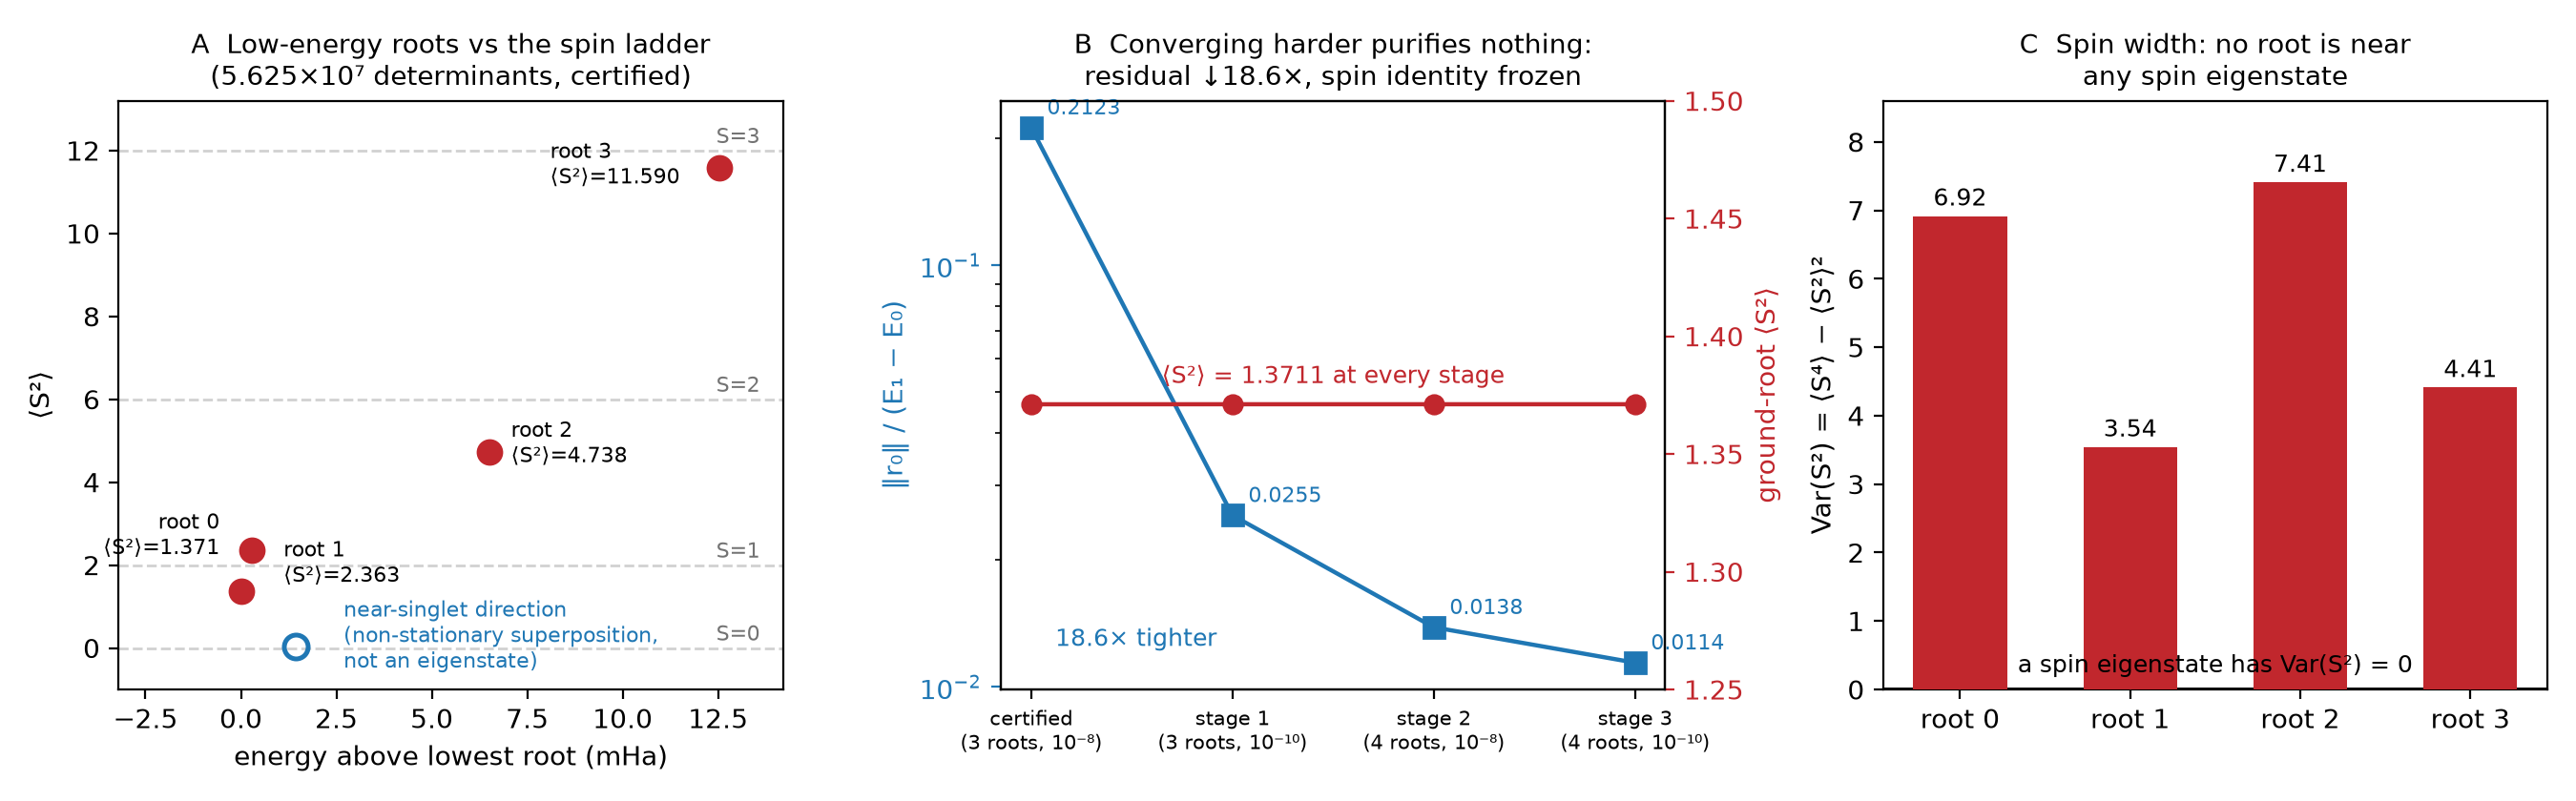
\includegraphics[width=\textwidth]{fig_flagship_s4.png}
\caption{The certified flagship-dimension subspace ($5.625\times10^7$ determinants, reconstructed here), four lowest roots. \textbf{A:} \ssq{} vs energy above the ground root, with pure-spin rails at $S(S+1)=0,2,6,12$; the near-singlet direction (open circle) is a non-stationary superposition 1.4~mHa above the minimum, not an eigenstate. \textbf{B:} across the stage-3/stage-4 certification the ground residual-to-gap ratio falls 18.6-fold ($0.2123 \to 0.0114$) while the ground-root \ssq{} holds at 1.3711. \textbf{C:} $\mathrm{Var}(S^2)$ per root; a spin eigenstate has $\mathrm{Var}(S^2)=0$, so no low-lying root is near one. Root~3 ($\ssq=11.59$) is the iteration-capped Ritz vector (Methods), the high-residual point in B, plotted as returned.}
\label{fig:flagship}
\end{figure}

\textbf{The kernel closed out: an independent implementation at the flagship dimension.} Every flagship number above, the solve and its certification alike, flows through one kernel: PySCF's \texttt{kernel\_fixed\_space}, the same matrix-free selected-CI engine the shipped solver wraps. Earlier drafts flagged that single-kernel dependence as a limitation; we closed it with a second implementation sharing no Hamiltonian-construction or solver code with the first. The Hamiltonian over the identical $5.625\times10^7$-determinant subspace was built explicitly by PyCI as a 1.6~TB on-disk sparse triangle whose nonzero count, \textbf{127{,}975{,}471{,}122, lands exactly on the closed-form combinatorial prediction: twice, in two independent builds on two fresh cloud instances}, and the eigenproblem was solved by our own block Davidson over our own threaded matrix--vector kernels (Methods). Three results. \emph{First}, the certified stage-4 vectors are eigenvectors of the independently built operator at machine precision: their Rayleigh quotients match the certified energies to $|\Delta| = 1.4\times10^{-14}, 2.0\times10^{-13}, 1.3\times10^{-13}$~Ha, a statement of kernel independence that requires no solver at all. \emph{Second}, perturbed by a deliberate $10^{-5}$-scale per-component jitter (initial block residual $2.0\times10^{-1}$, energies ${\approx}14$~mHa off), the independent solver re-converges all three roots in 38 iterations: energies within $(0.4, 0.6, 0.8)\times10^{-9}$~Ha of the certified values, and the spin ladder at $\ssq = \textbf{1.371065, 2.362748, 4.737714}$, within $5.2\times10^{-5}$, $7.5\times10^{-4}$, and $3.0\times10^{-4}$ of the certified ladder. \emph{Third}, the residual honesty this paper demands of others, applied to itself: the independent solve stops at maximum residual $1.25\times10^{-5}$ (4.4\% of the 0.285~mHa ground gap; a pre-registered wall-clock budget, with the diagonal preconditioner's slow tail against the near-degenerate pair documented in the run logs), so Davis--Kahan-type bounds permit intra-pair rotation up to $\sin\theta \approx 0.044$, bounding eigenvalue error by $5.5\times10^{-7}$~Ha and \ssq{} mixing by $1.9\times10^{-3}$. Every observed deviation sits inside its bound (energies by ${\sim}700\times$, spin by $2.5\times$). At the flagship dimension, two implementations sharing no code agree on the manifold, its energies, and its spin identity to the precision either can state: the two-solver pattern maintained at every rung $n \le 2000$ now extends to the published frontier.

\subsection{Cross-instrument certification and numerically certified sector bounds}\label{sec:crossinst}

\textbf{The instrument turned on its own output states.} For the final states of the [2Fe-2S] hardware, template, and set-draw legs and of the [4Fe-4S] hardware leg (mitigation on and off in each, eight arms in all), our independent $S^2$-Gram instrument (Section~\ref{sec:instrument}) agrees with the shipped \texttt{SCIState.spin\_square()} to better than $3\times10^{-14}$: the two implementations compute the same observable on the same states. We then push the moment ladder two rungs past the mean, to $\langle S^6\rangle$ and $\langle S^8\rangle$, by the same $M_s=0$ $S^+$-ladder identities, gauged on H4 FCI through the fourth moment \emph{and} on pure high-spin $S = 3/4/5$ reference states (built as the top eigenvector of PySCF's own \texttt{contract\_ss} $S^2$ operator, independent of the $S^+$ kernel; they exercise the third and fourth raising steps the H4 gauge cannot reach; Methods), and feed each state's measured moments to a linear program over the \emph{full} physical sector grid ($S = 0\ldots5$ for [2Fe-2S], $0\ldots9$ for [4Fe-4S]), returning moment-constrained sector bounds: numerically certified min/max weights for every sector (LP feasibility at tolerance $10^{-7}\cdot$scale; ``certified'' here means feasible-set bounds under those tolerances, not an analytic proof). This replaces the two-moment sector assumption with measurement. A nonnegative reading from $\ssq$ and $\langle S^4\rangle$ alone is only feasible, not unique: for the set-draw state a $\{0,1,3\}$ mixture with 60\% triplet weight reproduces its first two moments exactly, and the two-moment feasible set permits a triplet weight as high as 0.86. The third moment discriminates decisively: that alternative predicts $\langle S^6\rangle = 120$, the state measures $\langle S^6\rangle = 72.30$, and adding this one moment collapses the certified triplet ceiling to $8.4\times10^{-5}$ (the fourth moment $\langle S^8\rangle = 434.1$ tightens it to $3.0\times10^{-5}$). The full linear program over all physical sectors then pins the decomposition to $w_0 = 0.665$ (singlet) and $w_2 = 0.335$ (quintet), with the triplet weight below $4\times10^{-5}$ and the combined $S\ge3$ weight below $2\times10^{-5}$: the ``$2{:}1$ singlet--quintet'' reading is measured in full, not inferred from the mean (Table~\ref{tab:xinstr}).

\begin{table}[ht]\centering\small
\caption{Moments and numerically certified sector bounds of the eight final pipeline states. Two arms share $\ssq\approx2.00$; the higher moments and the linear-program triplet weight $w_1$ (numerically certified over all physical sectors) separate the genuine triplet from the singlet--quintet mixture.}
\label{tab:xinstr}
\resizebox{\textwidth}{!}{\begin{tabular}{lrrrrrl}
\toprule
leg (\texttt{symmetrize\_spin}) & \ssq & $\langle S^4\rangle$ & $\langle S^6\rangle$ & $\mathrm{Var}(S^2)$ & $w_1$ (LP, all $S$) & reading \\
\midrule
{[2Fe-2S]} hardware, on & 0.235 & 1.412 & 8.50 & 1.357 & ${<}\,10^{-4}$ & contaminated \\
{[2Fe-2S]} hardware, off & 0.231 & 1.205 & 6.95 & 1.152 & 0.024 & contaminated \\
{[2Fe-2S]} template, on & 0.108 & 0.650 & 3.96 & 0.638 & ${<}\,2\times10^{-4}$ & contaminated \\
{[2Fe-2S]} template, off & 0.123 & 0.705 & 4.29 & 0.690 & 0.006 & contaminated \\
{[2Fe-2S]} set-draw, on & 2.008 & 12.047 & 72.30 & 8.016 & ${<}\,10^{-4}$ & singlet--quintet mix, \emph{no} triplet \\
{[2Fe-2S]} set-draw, off & 1.089 & 2.693 & 9.92 & 1.507 & 0.498 & contaminated \\
\textbf{{[4Fe-4S]} hardware, on} & \textbf{2.000} & \textbf{4.000} & \textbf{8.00} & $\mathbf{3\times10^{-6}}$ & \textbf{1.000} & \textbf{triplet eigenstate, to tol.\ ($S=1$)} \\
{[4Fe-4S]} hardware, off & 3.003 & 18.048 & 144.73 & 9.028 & 0.450 & broad mixture, ${\ge}\,5\%$ at $S\ge3$ \\
\bottomrule
\end{tabular}}
\end{table}

Two arms converge to $\ssq\approx2.00$ and each could be reported as ``the triplet'' on the scalar mean alone; the higher moments separate them, and the linear program makes the separation numerically certified. The [4Fe-4S] hardware state (mitigation on) is a triplet eigenstate to measured tolerance: $\mathrm{Var}(S^2)=3\times10^{-6}$, and the LP pins its triplet weight to $w_1=1.000$ over all sectors $S\le9$ (the variance alone gives a Chebyshev cap of $\mathrm{Var}/4\approx7\times10^{-7}$ on non-triplet weight), so there the mitigation truly purifies (from $\mathrm{Var}(S^2)=9.0$ unmitigated), into the wrong sector. The [2Fe-2S] set-draw state (mitigation on) is not a triplet at all: its third moment numerically bounds the triplet weight below $10^{-4}$ across every physical sector (LP ceiling $8.4\times10^{-5}$), so the $2{:}1$ singlet--quintet reading is measured rather than assumed: the mean at 2.0 is a coincidence, and the 60\%-triplet alternative that the first two moments permit is excluded by the third. The other five [2Fe-2S] arms are broad low-spin mixtures ($\mathrm{Var}(S^2)=0.6$--$1.5$, LP triplet weight ${\le}\,0.5$); the unmitigated [4Fe-4S] arm is a broad high-spin mixture carrying a certified ${\ge}\,5\%$ weight in sectors $S\ge3$. This is the paper's own instrument turned on its own eight output states: a scalar \ssq{} labels none of them, and exactly one of the eight is a spin eigenstate to measured tolerance: the wrong one. (Full $\langle S^8\rangle$ per arm and the complete per-sector LP bounds are archived in \texttt{s6moments.npz}.) The bounds are additionally stress-tested against their own tolerance boxes: the box is a per-moment uncertainty interval ($10^{-7}\cdot\max(1, |m_k|)$), so the LP is an uncertainty propagation, and inflating every box $10\times$ and $100\times$ moves the set-draw triplet ceiling only from $3.1\times10^{-5}$ to $3.7\times10^{-5}$ and $1.0\times10^{-4}$, confines its singlet weight to $[0.6653, 0.6654]$, and leaves the [4Fe-4S] triplet floor above 0.99998: the sector readings are properties of the measured moments, not of tight tolerances (\texttt{\_s6stress.py}, \texttt{s6stress.npz}; all eight states, factors to $1000\times$).

\section{Discussion}\label{sec:discussion}

\textbf{What the controversy is actually about.} Both positions treat ``the energy at subspace size $D$'' as the benchmark quantity. Our audit shows that on the iron--sulfur systems this quantity does not identify a state: the low-energy manifold is a dense spin ladder, truncated-CI selection has a measured, persistent bias toward compact high-spin mixtures, and both quantum-sampled and classically-selected subspaces converge unidentified spin-contaminated mixtures. The critique's ``good guess vs bad guess'' framing dissolves (both guesses hit the same attractor); the flagship protocol does not produce the named singlet in any audited realization (and its mitigation measurably does not repair this). At the accuracy scale where the two camps disagree (a few mHa to a few tens of mHa), the spin-identity error is the \emph{same size as the disagreement}, so the controversy is undecidable on energies alone. This, we believe, is the real content of the dispute, and it is resolvable: measure the state.

\textbf{What each audited source claimed, and what we measured.} Because the critique is aimed at published claims, its scope should be explicit. Table~\ref{tab:claims} places each audited source's own words beside the state diagnostic it reported and what this audit establishes. Setting the claims side by side forecloses the objection that we contest a stronger statement than was made: the variational upper bound is \emph{granted}; it is a true statement about an energy (see ``What the energy still means,'' below), and what is shown unmet is the state identity each source either names or leaves unmeasured. The pattern is uniform. The one source that names a spin target (the flagship: ``singlet states \ldots\ eigenfunctions of total spin with eigenvalue 0'') reports an energy but never an \ssq{}; the spin-handling mechanisms the sources invoke (``closure under spin inversion,'' plus, for the flagship, the stated soft-constraint penalty at $\lambda=0.2$) are the ones Section~\ref{sec:mitigation} measures: closure permits but does not produce a singlet, and the stated penalty, in its shipped linear form and its stated squared form alike, yields no competitive singlet, reaching one at best at the subspace's $+2.9$~Ha floor; and the full-scale successor that carries the program past our audit reach names no spin target and reports no spin diagnostic at all.

\begin{table}[!ht]\centering\footnotesize
\setlength{\tabcolsep}{4pt}
\renewcommand{\arraystretch}{1.15}
\caption{Claim alignment across audited sources. Each row pairs a source's own stated claim (verbatim in quotation marks) with the state diagnostic it reported and what this audit establishes. No audited source that names a spin target reports a spin diagnostic for its computed states; the invoked spin-handling mechanisms, closure under spin inversion and the flagship's stated soft-constraint penalty, are measured in Section~\ref{sec:mitigation}.}
\label{tab:claims}
\begin{tabular}{p{2.6cm}p{3.4cm}p{2.1cm}p{2.4cm}p{3.5cm}}
\toprule
\textbf{Source} & \textbf{Stated claim (verbatim in quotes)} & \textbf{Names a spin target?} & \textbf{State diagnostic reported} & \textbf{What this audit establishes} \\
\midrule
\textbf{IBM flagship}, arXiv:2405.05068 (Sci.\ Adv.\ 2025) & ``upper bounds for the ground-state energy'' and ``sparse approximations to the ground-state wavefunctions'' for systems ``beyond sizes amenable to exact diagonalization'' & \textbf{Yes}: computed ``in the $S_z=0$ and $S^2=0$ subspace,'' targeting ``singlet states \ldots\ eigenfunctions of total spin with eigenvalue 0'' & Energy only; no \ssq{}. Spin handled by ``approximate restoration of the $S^2$ symmetry \ldots\ closure under spin inversion'' plus ``a soft constraint in the eigenstate solver \ldots\ to mitigate spin contamination'' ($H+\lambda[S^2-s(s+1)]^2$, $\lambda=0.2$) & The upper bound stands as a statement about an energy; but the audited trajectories and the reconstructed flagship subspace carry \ssq{} from 1.37 upward, never the singlet's 0; spin-inversion closure permits but does not produce the named singlet; and the stated constraint, run at its stated form and strength on the benchmark-energy subspace, yields no competitive singlet in either compression (the projected square holds $\ssq = 3.01$ at $+528$~mHa; the literal square $P(S^2)^2P$ reaches a singlet only at the $+2.9$~Ha floor) (Secs.~\ref{sec:mitigation}, \ref{sec:flagship}). The reported energy is not identified with the singlet. \\
\midrule
\textbf{IBM data archive}, zenodo.15324153 & Released hardware shots, noiseless-template samples, uniform controls, and a recovery ablation for the demonstrations above & N/A (released data) & Energies; no per-state \ssq{} & Direct archive result: the archive's own inputs, run through the shipped pipeline, populate a spin--energy vise: benchmark-grade energy only at $\ssq=4.8$, or low scalar \ssq{} only at $+229$--$248$~mHa (where the raw hardware shots land), never both (Secs.~\ref{sec:archive}--\ref{sec:rawladder}); the authors' own recovery ablation attributes the accuracy to the classical post-processing (Sec.~\ref{sec:archive}). \\
\midrule
\textbf{Shipped software}, \texttt{qiskit-\allowbreak addon-\allowbreak sqd} (tested 0.3.0--0.12.1) & Diagonalizes sampled subspaces; offers a \texttt{symmetrize\_spin} closure and a \texttt{fix\_spin\_} penalty; exposes \texttt{SCIState.\allowbreak spin\_square()} & Optional: spin symmetrization and penalty are available but \textbf{off by default} & \ssq{} obtainable via \texttt{spin\_square()} but not invoked on the default path; the solver can return \texttt{converged=\allowbreak False} without raising & Version-tested behavior: \texttt{symmetrize\_spin} changes the result by ${<}\,1$~nHa on realistic spin-mixed input (a no-op exactly where it is needed), the default path measures no spin, and the penalty is off by default (Secs.~\ref{sec:mitigation}, \ref{sec:theirsamples}). \\
\midrule
\textbf{RIKEN--IBM successor}, arXiv:2511.00224 (Nov 2025) & Closed-loop SQD to $D\approx10^{10}$ with ``accuracy comparable to some all-classical approximation methods,'' ``beyond the reach of exact diagonalization'' & \textbf{No}: ``singlet'' and ``triplet'' occur once each, inside the title of a cited reference; no \ssq{} & Energy and energy variance; no spin diagnostic. Mitigation $=$ mirror symmetrization with the Hartree--Fock string ``manually added'' & Not directly spin-audited ($D\ge10^9$ is beyond our reach; Limitations item~1). Inheritance argument only: the same product-space completion and the same energy-only identification, so the same gap applies unless a spin measurement shows otherwise (Sec.~\ref{sec:discussion}, ``The full-scale successor inherits the gap''). \\
\bottomrule
\end{tabular}
\end{table}

The alignment is deliberately narrow. It does not claim that no SQD execution could ever return the named singlet, nor that the unpublished flagship eigenvector was definitely contaminated; it establishes that on every execution this audit could reach (trajectories, shipped pipeline, released hardware shots, and the reconstructed flagship-dimension subspace), the returned state carries the spin width the reported energies never disclosed.

\textbf{The structural mechanism.} The pattern has a one-line root: determinant selection is a projector $P$ that is not $S^2$-invariant, so although $[H, S^2] = 0$ exactly, the compressed operators need not commute, $[PHP,\, PS^2P] \neq 0$, and the eigenbasis of $PHP$ need not align with any spin sector. Every spin-identity finding in this audit is a face of that noncommutation: the compactness bias (the ground state of $PHP$ optimizes energy in a space where spin sectors mix), the permits-vs-produces failure of spin-inversion closure (closure constrains the support of $P$ but does not make $PS^2P$ commute with $PHP$; Section~\ref{sec:mitigation} measures the consequence), and the flagship-dimension manifold whose near-singlet direction is not an eigenstate (Section~\ref{sec:flagship} exhibits the two compressed $3\times3$ blocks directly, and its second-moment audit measures every low root at $\mathrm{Var}(S^2) \ge 3.5$: spin width, not spin labels). (The sampling wall of Section~\ref{sec:nowin} is a distinct mechanism: distribution concentration, not broken commutation, and bounds support recovery, not state identity.) The noncommutation also separates three conditions that benchmark practice routinely conflates: (i) the target state is \emph{representable} in the subspace; (ii) target character is \emph{present} within the low-energy manifold; (iii) the eigensolver \emph{returns} the target as an eigenstate. Only the third supports a named-state energy. Spin-inversion completion achieves the first (Section~\ref{sec:mitigation}); the flagship Gram audit exhibits the second, a near-singlet direction inside the certified low-energy span (Section~\ref{sec:flagship}); neither delivers the third. Eliminating the noncommutation requires an $S^2$-invariant construction: spin-adapted (CSF) bases or $S^2$-projected selection, for which $[PHP,\, PS^2P] = 0$ by construction. A solver-side penalty is not such a construction: adding any function of $PS^2P$ (the linear $\lambda PS^2P$, or the flagship's stated squared $\lambda[PS^2P]^2$) does not change $P$, and it commutes with $PS^2P$, so the noncommutation with the projected energy is unaltered; the penalty reshapes the spectrum of $PHP$ and biases its ground state toward whatever low-spin directions the selected space already represents, which is why it can target a singlet only once selection has placed a competitive one in the subspace (Section~\ref{sec:mitigation} measures both forms landing on the same wall). This is what the recommendations below amount to.

\textbf{What the energy still means.} Spin contamination does not erase the variational meaning of the energy; it erases the state-specific meaning assigned to it. A contaminated $M_s = 0$ root remains a variational upper bound on the global ground-state energy and may be quoted as one; what it cannot support is identification with the named singlet: its energy, its wavefunction, or any observable of the spin ladder read from it.

\textbf{The full-scale successor inherits the gap.} While this audit was under way, the flagship program scaled again: a RIKEN--IBM collaboration (arXiv:2511.00224, November 2025) reports closed-loop SQD on [2Fe-2S] (50e,\,36o; a larger active space than the [2Fe-2S] benchmark audited here) and [4Fe-4S] (54e,\,36o; its DMRG reference, $-327.239$~Ha, matches the benchmark dump's to the milli-Hartree, so on this system the successor and our audit address the same spectrum) at subspace dimensions up to $10^{9}$--$10^{10}$ on Fugaku, improving the best [4Fe-4S] energy to $-326.912$~Ha at $D=10^{10}$ and extrapolating in the energy--variance plane to $-327.118\pm0.02$~Ha, a value its own text notes ``deviates by about 0.12~$E_{\mathrm{h}}$'' from the DMRG reference. Three features, each verifiable from its full text, place the successor inside this paper's critique rather than beyond it. (i)~It reports no spin measurement of any kind: in its full text, ``singlet'' and ``triplet'' each occur exactly once, inside the title of a cited reference, and no \ssq{} or spin diagnostic appears; the computed state is identified by energy alone. (ii)~Its spin mitigation is the mechanism this paper measures failing: mirror symmetrization of the sampled $\alpha/\beta$ half-configurations, with the Hartree--Fock string ``manually added'' when sampling misses it, the same product-space completion whose ground manifold contains no singlet at any scale we audited (Sections~\ref{sec:mitigation}, \ref{sec:theirsamples}). (iii)~Its classical baselines are CCSD and the DMRG reference; no selected-CI baseline at matched subspace dimension is run, so the matched-dimension question of Section~\ref{sec:nowin} is not answered at $10^{10}$: it is unexamined there. Finally, the successor's central accuracy argument (extrapolation to zero energy variance) does not substitute for state identification: extrapolating the energies of unidentified states targets whichever eigenstate the trajectory approaches, and a terminal 0.12~Ha gap from DMRG is exactly the signature an energy-only protocol cannot diagnose, because slow convergence toward the singlet and faithful convergence toward a different, unidentified eigenstate are indistinguishable without a spin measurement. One sparse matrix--vector product per reported state would settle it. This inheritance argument has definite limits. It is an argument from shared mechanism and shared data handling, not a spin measurement of the successor's own states, which at $10^{9}$--$10^{10}$ remain beyond our audit (Limitations item~1), and the paper does not rest on it: the load-bearing findings are the fully-measured lower-dimension results on their own integrals, subspaces, hardware shots, and shipped pipeline (Sections~\ref{sec:archive}--\ref{sec:crossinst}), which identify the failure directly and stand whether or not the successor is ever audited at scale.

\textbf{Boundary theory: where quantum samples could still matter.} Our results close the matched-dimension question in every regime we could reach exactly (equilibrium, stretched, diradical; three certified implementations; three seeds) and add the flagship-scale identity failure. The surviving candidate value of quantum sampling is not accuracy-per-determinant but \emph{escape dynamics}: selection hysteresis is real (Section~\ref{sec:retraction}), and samples from a state on the correct potential-energy sheet cannot be trapped by a wrong-state seed. But this value is only realizable if the circuit prepares (approximately) the right state, and the flagship initialization measurably does not at exactly the near-degeneracies where escape matters (CCSD-seeded LUCJ at the diradical: 181 unique determinants, $+64$~mHa, wrong-state bias inherited from CCSD). A quantum advantage claim for SQD therefore requires, at minimum: (i) a demonstrated preparation whose sample distribution favors the \emph{named} target state where classical selection demonstrably follows a different one, and (ii) spin (and other symmetry) identification of every reported state. Neither exists in the current literature.

\textbf{A falsifiable challenge.} Our claims fail if anyone can exhibit: (1) a quasi-degenerate ground manifold (Methods: $\Delta E < 2\,\mu$Ha) of a spin-completed subspace of these benchmark systems whose $S^2$-Gram floor is $< 1$ (target 0), using the Gram instrument provided; rotations across gaps far larger than the degeneracy window are superpositions, not eigenstates, and do not qualify (the certified flagship manifold of Section~\ref{sec:flagship} illustrates the distinction: ground-pair floor 1.371; its $\ssq = 0.038$ direction exists only as a non-stationary mixture across a 6.5~mHa gap); (2) a quantum-sampled subspace at matched determinant count whose \emph{spin-identified} ground-state energy beats HCI/CIPSI on any system here; or (3) a run of the shipped pipeline, on any sample source in IBM's own archive, that escapes the spin--energy vise ($\ssq < 1$ \emph{and} error $< 50$~mHa on [2Fe-2S]), with or without a solver-side spin penalty (we measured that a solver-side penalty does not escape it: the shipped linear \texttt{fix\_spin\_} at and beyond its default, and the flagship's stated squared constraint at its stated $\lambda = 0.2$ alike: the benchmark-energy subspace reaches a singlet only 2.9~Ha up, Section~\ref{sec:mitigation}; escaping via spin-aware \emph{selection} would confirm our recommendation, not refute our claim). The harnesses are in the supplementary archive.

\textbf{Recommendations.} (1) Every selected-CI-family benchmark (classical or quantum-sampled) on open-shell systems should report determinant-space \ssq{} (and, within quasi-degenerate manifolds, the invariant $S^2$-block eigenvalues) for every state whose energy is reported. The cost is negligible. Spin moments are the first identity certificate, not the complete one: in a dense exchange ladder a spin-pure root can still be the wrong root of its sector, so a full certificate adds the remaining symmetries and target diagnostics the named state defines (spatial irreducible representation, particle number, overlap or root continuity against a declared target, and an energy becomes state-specific only when the returned eigenvector passes the certificate declared in advance. (2) Spin control should be \emph{active}, not passive, and active at \emph{selection}, not only at diagonalization. Subspace completion alone is measurably insufficient (Section~\ref{sec:mitigation}), and so is a spin penalty applied after the fact to a marginal-product subspace: switched on, in the shipped linear form or the flagship's stated squared form, it reaches a singlet only 2.9~Ha above the reference because the sampled subspace contains no competitive singlet (Section~\ref{sec:mitigation}). Spin-adapted CSF bases or $S^2$-projected selection that retains the recoupling determinants are the level at which the fix must act; a \texttt{fix\_spin\_}-style penalty then targets the singlet within a subspace that actually contains one. (3) Matched-dimension discipline (every quoted $D$ = the dimension actually diagonalized) should be standard in QSCI/SQD comparisons, as the first-order cost axis, not the whole cost model: connectivity, product-space structure, and solver internals also set wall-clock and memory, which is why our Methods reports iteration counts, wall times, and peak memory per leg. (4) Iron--sulfur ``beyond exact'' claims should be re-stated as energies of identified states, or explicitly rescoped as probe-regime results.

\FloatBarrier
\section{Methods}

\textbf{Terminology: four senses of ``certified.''} This paper uses the word in four distinct senses, each disambiguated by context and none implying the others: \emph{residual-certified}: an eigenpair met a stated solver tolerance, quoted together with its measured residual and the local gap that residual must be compared against; \emph{cross-kernel reproduced}: re-derived by an independent implementation (the PyCI-built operator and in-house eigensolver of Section~\ref{sec:flagship}); \emph{numerically certified}: an LP min/max over the moment-feasible set at stated tolerances (defined at its first use in the flagship-leg paragraph below), not an analytic bound; and \emph{artifact-verified}: a manuscript statement re-derived from the archived outputs by \texttt{\_paperaudit.py} (internal consistency only; see ``Automated claim verification'').

\textbf{Certification chain.} All Hamiltonians are read from the public Li--Chan FCIDUMPs ([2Fe-2S]: 20 orbitals, 30 electrons; [4Fe-4S]: 36 orbitals, 54 electrons). Our Slater--Condon engine, PySCF, and PyCI agree to $\mu$Ha on diazene FCI cross-checks; production iron--sulfur ladders use PyCI (\texttt{add\_hci} with $\varepsilon$-ladder factor $10^{-0.1}$, \texttt{sparse\_op.solve} to $10^{-9}$). Our HCI implementation independently reproduces the critique's published N$_2$ HCI curve. PySCF's own SCI independently reproduces the diazene triplet trap. The [2Fe-2S] 170k-determinant space re-solves to the recorded energy exactly on reload (stage-1 check of the as-shipped test).

\textbf{Spin audit.} \ssq{} and $S^2$-Gram blocks computed as in Section~\ref{sec:instrument}, with the diazene gauge gate (known triplet/singlet/singlet labels; required diagonal $(2,0,0)$, off-diagonals $<10^{-6}$) run before every production audit. Quasi-degenerate clusters defined by $\Delta E < 2\times10^{-6}$~Ha. That convention sits on a measured plateau (\texttt{\_thrscan.py}, \texttt{thrscan.npz}): re-deriving every cluster partition from the archived root energies (49 stored root vectors (138 roots) across the trajectory, completion, completion-mechanism, and flagship records) reproduces the production partition exactly at 0.2~$\mu$Ha, at 2~$\mu$Ha, and under a residual-adaptive criterion (roots cluster when their gap falls below the per-root eigenvalue uncertainty: the solve tolerance where residuals are not archived, the Kato--Temple-style $r^2/\mathrm{gap}$ bound where they are), because the partition is set by a separation margin: the largest split inside any production cluster is $1.9\times10^{-12}$~Ha, the smallest gap between distinct clusters 4.8~$\mu$Ha, a $2.6\times10^6$-fold window around the convention. Only at 20~$\mu$Ha does exactly one assignment change: the two lowest roots of the [2Fe-2S] aufbau trajectory checkpoint at $D=5{,}053$ (gap 4.8~$\mu$Ha; per-root $\ssq=2.05$ and 2.07, both mid-mixture, the wandering point of Section~\ref{sec:fe2s2}) merge into a cluster the paper never reported as one; no completion pair, no flagship manifold, and no reported block spectrum is affected. Spin completion implemented as full spin-inversion closure of the determinant set, re-solved with identical solver settings.

\textbf{Sampling and matched dimension.} Sampling arms draw multinomial shots from $|c|^2$ of the stated vector (exact-distribution arms) or from LUCJ circuit simulation (ffsim, CCSD $t_2$ initialization, with determinant-mapping self-tests). Classical growth uses $\times1.5$ incremental selection with full re-solve so that every reported $D$ is the diagonalized dimension. Diazene comparisons use $B=2\times10^6$ shots and three RNG seeds.

\textbf{As-shipped pipeline.} We call \texttt{diagonalize\_fermionic\_hamiltonian} from \texttt{qiskit-addon-sqd} (installed release) with \texttt{samples\_per\_batch}=500, \texttt{norb}=20, \texttt{nelec}=(15,15), \texttt{num\_batches}=3, \texttt{max\_iterations}=4, \texttt{symmetrize\_spin}$\in\{$\texttt{True},\texttt{False}$\}$, \texttt{max\_dim}=500, \texttt{seed}=17; bitstrings packed $[\beta\ldots,\alpha\ldots]$ per its convention; $10^6$ multinomial shots from the $D=170{,}448$ aufbau vector; energies reported with ECORE = 0 (per the FCIDUMP); \ssq{} from \texttt{SCIState.spin\_square()}. Per-batch trajectories in \texttt{sqdship\_symm1.npz} and \texttt{sqdship\_symm0.npz}. The published-construction ladder of Section~\ref{sec:rawladder} uses the same driver on the reconstructed 2{,}457{,}600-shot hardware BitArray with \texttt{samples\_per\_batch} $= 3N$, \texttt{num\_batches} $= 10$, \texttt{max\_iterations} $= 5$, \texttt{max\_dim} $= N \in \{500, 1000, 2000\}$, seed 17 (seed 43 and \texttt{symmetrize\_spin=False} ablations at $N=1000$; an independent same-configuration run of $N=500$ on second hardware), energies vs the same reference; per-batch trajectories in \texttt{sqdraw\_n\{N\}\_\{arm\}\_s\{seed\}.npz}.

\textbf{Penalty-on audit (Section~\ref{sec:mitigation}).} \texttt{\_sqdpen.py}. We first captured the shipped off-arm subspaces by rerunning \texttt{diagonalize\_fermionic\_hamiltonian} on the $10^6$ soup-vector samples at the Section~\ref{sec:mitigation} knobs (\texttt{samples\_per\_batch}=500, 3 batches, \texttt{max\_dim}=500, 4 iterations, seed 17), saving every iteration's product-space CI strings; the best space ($D=441^2$) reproduces the published $-116.560107$~Ha / $\ssq=4.834$ and the iteration-1 space ($D=245^2$) reproduces $-116.515503$~Ha / 4.903. On each fixed space we solved the ground state of $H+\lambda S^2$ by Lanczos (\texttt{scipy.sparse.linalg.eigsh}, $k=1$, \texttt{ncv}=64) whose matrix--vector products call PySCF's own \texttt{selected\_ci.contract\_2e} (for $H$, via \texttt{absorb\_h1e}) and \texttt{contract\_ss} (for the projected $S^2$)), the exact operators \texttt{fix\_spin\_} penalizes and \texttt{spin\_square} measures, over the penalty grid $\lambda \in \{0, 0.1, 0.2, 0.5, 1, 2, 5, 20\}$, warm-started by continuation, reporting the true energy $\langle H\rangle$ (from the RDMs), \ssq, and $\mathrm{Var}(S^2)$ of each converged root with its explicit residual ($\leq 9\times10^{-8}$). At $\lambda=0$ the eigensolver reproduces the shipped record and agrees with an independent PyCI diagonalization of the identical determinant space to 0.00~$\mu$Ha; the singlet-sector endpoint (large $\lambda$; $\ssq=\mathrm{Var}(S^2)=0.0000$, an exact singlet by positive-semidefiniteness) is the lowest-energy exact singlet the subspace contains, corroborated by the lowest closed-shell determinant's diagonal energy as an independent single-determinant upper bound ($+3.05$~Ha; \texttt{\_sqdpen\_diagprobe.py}). We then reran their solver on the same fixed spaces exactly as \texttt{solve\_sci} wires it (\texttt{kernel\_fixed\_space} with \texttt{fix\_spin\_(ss=0, shift}$\in\{0.1,0.2\}$\texttt{)}, at the silent default \texttt{max\_cycle} and at \texttt{max\_cycle}=600; every one of the five arms returned \texttt{converged=False}, 0.27--0.33~Ha above the penalized minimum; seeded instead with our converged penalized vector, the same kernel returns \texttt{converged=True} at overlap 1.000000 and our exact penalized Rayleigh quotient (\texttt{\_sqdpen\_s3b.py}, \texttt{sqdpen\_s3b.npz}). Finally we reran the entire configuration-recovery protocol (same knobs and seed) with the penalty active ($ss=0$, converged eigensolver solves) at $\lambda=0.1$ and 0.2. Two companion runs solve the flagship's stated squared constraint, $H+\lambda[S^2-s(s+1)]^2$ at $s=0$ and $\lambda=0.2$, on the same captured $D=441^2$ space, in the two ways that operator compresses onto a fixed subspace (PySCF's \texttt{fix\_spin\_} implements only the linear shift, so both require a dedicated operator). \texttt{\_sqdpen\_sq.py} applies \texttt{contract\_ss} twice, the projected square $(PS^2P)^2$; \texttt{\_sqdpen\_true.py} builds the literal square $P(S^2)^2P$ from the exact $M_s=0$ spin ladder (sparse $S^+$ operators mapping $P$ to the $M_s{+}1$ and $M_s{+}2$ product spaces, so that $P(S^2)^2P\,c = R_1^{\mathsf T}(R_2^{\mathsf T}S_+^2 c + 2 S_+ c)$), gauged operator-for-operator against PySCF's \texttt{contract\_ss} and a dense projected $S^4$ to machine precision (the G0 gate) before the run. Both use Lanczos as above, warm-started, with the $\lambda=0$ anchor certified against the shipped record by the same gates. Outputs \texttt{sqdpen\_frontier.npz}, \texttt{sqdpen\_theirs.npz}, \texttt{sqdpen\_spaces.npz}, \texttt{sqdpen\_loop\_l\{10,20\}.npz}, \texttt{sqdpen\_sq\_it4.npz} (the projected-square point) and \texttt{sqdpen\_true\_it4.npz} (the literal-square point and its $\lambda$-sweep), each with final vectors; figure \texttt{fig\_penalty\_frontier.png} (\texttt{\_sqdpenfig.py}).

\textbf{Completion-mechanism audit (Section~\ref{sec:mitigation}).} \texttt{\_degen.py} rebuilds every spin-completion checkpoint of the three trajectory arms from the archived determinant sets (\texttt{s2audit\_*.npz}), re-solves the uncompleted and completed spaces with PyCI (lowest three roots, tolerance $10^{-9}$), and records per checkpoint: the ground-energy shift under completion; the completed ground-manifold splitting; the invariant spectrum of the original-support projector compressed over the ground manifold; the localized pair member's weight on the added determinants; the coupling $\|P_+ H v\|$ (the uncompleted ground embedded with zeros, the completed-space operator applied, the result projected onto the added determinants); and the invariant $S^2$ Gram block over the manifold (\texttt{degen.npz}). At the one checkpoint whose iterative record lacks a resolved pair ([4Fe-4S], $1{,}106 \to 2{,}097$), \texttt{\_degen\_dense.py} builds the full 2,097-dimensional Hamiltonian by explicit matrix--vector columns and diagonalizes it densely (LAPACK), restoring the exact degenerate pair and re-deriving the same row quantities gauge-invariantly; the iterative artifact (three distinct Ritz values, one per degenerate pair) is preserved in the same archive (\texttt{degen\_dense.npz}). Table rows and prose bounds are generated from these archives by \texttt{\_degen\_table.py}.

\textbf{Version matrix.} \texttt{\_verm.py} repeats the construction--solver--diagnostic semantics at the earliest publicly auditable release (0.3.0; we could not retrieve the stated 0.1.0 through PyPI or a tagged GitHub release as of 2026-07-15; Limitations item 7) and at 0.12.1, on identical inputs: the $N=60$ reproducer core, and a seed-17, 500-shot in-sector batch of the raw [2Fe-2S] hardware counts with closure on and off, each version through its own entry points (\texttt{bitstring\_matrix\_to\_sorted\_addresses} / \texttt{solve\_fermion(\ldots, max\_davidson=400)} at 0.3.0; \texttt{bitstring\_matrix\_to\_ci\_strs} / \texttt{solve\_fermion(\ldots, max\_cycle=400)} at 0.12.1). Outputs \texttt{verm\_0\_3\_0.npz} / \texttt{verm\_0\_12\_1.npz}.

\textbf{Flagship-dimension leg (Section~\ref{sec:flagship}).} Outer-product subspaces from the top-$N$ of the 7{,}658 released unique half-configurations per spin, ranked by the exact marginals of the rebuilt optimized-circuit state (\texttt{lucjopt\_marginals.npz}; the released strings load as uint64 and must be cast to int64 and sorted before use). Solver: \texttt{qiskit\_addon\_sqd.fermion.solve\_fermion} on their MO FCIDUMP, as shipped, cold-started, with \texttt{max\_cycle=400} and \texttt{verbose=5} forwarded to PySCF (the shipped default \texttt{max\_cycle} would return an under-converged flagship energy without warning; no other kwarg is set and \texttt{spin\_sq} is left unset so the reported \ssq{} is their code's own). Rungs $N \in \{300, 500, 600, 1000, 2000\}$ are certified against PyCI anchors on the identical construction ($\Delta E$ 0.002--0.023~mHa; the $n=600$ rung also reproduces the exact cross-implementation reconstruction energy to 0.08~$\mu$Ha). The $N=7500$ rung (their published $5.625\times10^7$) ran 63{,}846~s at 32 threads on a 64-vCPU \texttt{c7i.16xlarge} (peak RSS 13.6~GB), 400 Davidson iterations to final residual $3.5\times10^{-4}$. Full amplitude matrices and string sets are archived in \texttt{flagsolve\_n\{N\}.npz}; the $N=2000$ rung was additionally converged on two further platform/thread configurations (\texttt{flagsolve\_n2000\_box1.npz}), yielding the \ssq{} run-instability datum; per-attempt cloud logs (\texttt{flagsolve\_box1\_attempt\{1,2,3\}\_live.log}) document three spot-instance interruptions with no data loss (2-minute result syncing). The flagship rung was subsequently certified by a dedicated three-root block eigensolve of the identical subspace (\texttt{pyscf.fci.selected\_ci.kernel\_fixed\_space}, \texttt{nroots = 3}; the same matrix-free kernel \texttt{solve\_fermion} wraps), warm-started from the banked flagship vector under three pre-registered gates (bit-identical string sets; warm-vector Rayleigh quotient vs banked energy, measured 0.0~$\mu$Ha; warm \ssq{} vs banked, $<10^{-14}$), initial block $=$ warm root plus two lowest-diagonal guesses, tolerance ladder $10^{-6}/10^{-7}/10^{-8}$ (\texttt{max\_cycle} 150/150/200), with the $S^2$-Gram audit and a full checkpoint after each stage; all three roots met the solver's per-root convergence criteria, final residuals $(6.0, 8.4, 9.1)\times10^{-5}$ (the tightest still 21\% of the 0.285~mHa ground gap; see the stability-vs-residual discussion in Section~\ref{sec:flagship}); 11.3~h at 64 threads on a 64-core \texttt{c7a.16xlarge}, peak RSS 41.8~GB. Script \texttt{\_gram7500.py}, log \texttt{gram7500.run.log}, per-stage summaries \texttt{gram7500\_ck\{1,2,3\}.npz}, final \texttt{gram7500.npz}; the converged three-root vector block \texttt{gram7500\_restart.npz} (1.3~GB) ships as a Zenodo companion beside the flagship amplitudes. The stage-4 follow-up (\texttt{\_gram7500s4.py}; 14.8~h at 64 threads on the same instance class, peak RSS 43.7~GB) warm-starts from that certified block under the same gates plus an in-box moment gauge (H$_4$/STO-3G FCI: per-eigenstate $|\mathrm{Var}(S^2)| < 10^{-9}$ and an analytic two-state mixture variance reproduced to $10^{-9}$, asserted before production; standalone version \texttt{\_s4gate.py}), grows the block with orthogonalized lowest-diagonal guesses, and re-solves through stages (\texttt{nroots}, \texttt{tol}, \texttt{max\_cycle}) $=$ $(3, 10^{-10}, 120)$, $(4, 10^{-8}, 150)$, $(4, 10^{-10}, 150)$, re-measuring energies, residuals, the $S^2$-Gram, and the $S^4$ moments after every stage (checkpoints \texttt{gram7500\_s4ck\{0--3\}.npz}, final \texttt{gram7500\_s4.npz}, run log \texttt{gram7500s4\_live.log}; the final four-root vector block \texttt{gram7500\_s4\_restart.npz}, 1.8~GB, ships as a Zenodo companion beside the three-root block). Second moments use the $M_s = 0$ identity: with $W = S^+V$ the deduplicated $S^+$-image of the root block and $W_2 = S^+W$, $G = W^{\mathsf{T}}W$ and $G_4 = W_2^{\mathsf{T}}W_2 + 2G$, so $\mathrm{Var}(S^2)$ per root is $(G_4)_{ii} - (G)_{ii}^2$; the $\{S = 0, 1, 2\}$ sector solve inverts the moment pair on the sector eigenvalues $\{0, 2, 6\}$ ($w_2 = (\langle S^4\rangle - 2\ssq)/24$, $w_1 = (6\ssq - \langle S^4\rangle)/8$, $w_0 = 1 - w_1 - w_2$), a negative weight certifying support outside $S \le 2$. The same gauged moment kernel is applied by \texttt{\_s4states.py} to the eight final pipeline states of the cross-instrument legs (Section~\ref{sec:crossinst}), each gated against the shipped \texttt{spin\_square} to $10^{-6}$ before its $\langle S^4\rangle$ and sector solve are recorded (\texttt{s4states.npz}). A follow-on kernel (\texttt{\_s6moments.py}) extends the same $M_s = 0$ $S^+$-ladder on those eight states to the third and fourth moments, $\langle S^6\rangle = |\phi_3|^2 + 8|\phi_2|^2 + 4|\phi_1|^2$ and $\langle S^8\rangle = |\phi_4|^2 + 20|\phi_3|^2 + 52|\phi_2|^2 + 8|\phi_1|^2$, with $\phi_k = (S^+)^k\psi$ built by chunked deduplication, gauged in-process two ways before production (both hard-asserted): on H$_4$/STO-3G FCI, every eigenstate closes as $\langle S^{2k}\rangle = \lambda^k$ and an analytic 0.7/0.3 singlet--triplet mixture reproduces $(\langle S^6\rangle, \langle S^8\rangle) = (2.4, 4.8)$ to $<10^{-9}$; and on pure maximum-spin $S = 3, 4, 5$ $M_s = 0$ reference states (built as the top eigenvector of PySCF's own \texttt{contract\_ss} $S^2$ operator, independent of the $S^+$ kernel), every measured moment closes as $\langle S^{2k}\rangle = [S(S+1)]^k$ ($k = 1\ldots4$) to $<10^{-6}$ relative. This second gauge exercises the third and fourth raising steps $\phi_3/\phi_4$, which the H4 gauge (whose FCI space caps at $S = 2$) never drives with nonzero vectors, so the [4Fe-4S] LP (which runs to $S = 9$) rests on verified moments at every rung it uses. The measured moments then constrain a linear program (\texttt{scipy.optimize.linprog}, HiGHS) over sector weights $w_S \ge 0$ on the full physical grid $S = 0\ldots S_{\max}$ ($S_{\max} = (2\,\mathrm{ncas} - \mathrm{nelec})/2$: 5 for [2Fe-2S], 9 for [4Fe-4S]), with the norm and each available moment enforced to tolerance $10^{-7}\cdot\text{scale}$, returning numerically certified min/max of the singlet, triplet, and combined $S \ge 3$ weights (throughout, ``numerically certified'' denotes the min/max over the LP-feasible set at these tolerances, not an analytic bound), plus the unique $\{0,1,2,3\}$ four-moment solve whose negative component would certify $S \ge 4$ support (\texttt{s6moments.npz}). Each state's $m_1$ is re-gated against the shipped \texttt{spin\_square} ($10^{-6}$) and its $(m_1, m_2)$ against the frozen \texttt{s4states.npz} values ($10^{-8}/10^{-6}$) before its bounds are recorded. A sensitivity companion (\texttt{\_s6stress.py}) re-runs the identical LP with every per-moment box inflated $10\times$, $100\times$, and $1000\times$, gating the factor-1 run against the production bounds before recording the inflated ones (\texttt{s6stress.npz}). Roots 0--2 meet the solver's per-root criteria at every stage (final measured residuals $(3.2, 4.1, 2.6)\times10^{-6}$); root 3 reaches the final stage's iteration cap with measured residual $3.3\times10^{-5}$ (energy stable to $<10^{-9}$~Ha per iteration over the closing ten); we therefore report its energy and moments as measured properties of the returned vector, without labeling that root converged.

\textbf{Independent-implementation flagship cross-check (Section~\ref{sec:flagship}).} \texttt{\_tb7500box.py} on a storage-optimized cloud instance (\texttt{i4i.16xlarge}: 64 vCPU, 512~GiB RAM, $4\times3.75$~TB NVMe in RAID-0). The $N = 7500$ outer-product subspace is rebuilt from \texttt{tb7500\_strings.npz} (hash-gated against the flagship payload), and the Hamiltonian over it is constructed by PyCI in 512 row-chunks across 20 worker processes (rectangular \texttt{sparse\_op} rows under a closed-form column map; global lower triangle, each pair stored exactly once), streamed to a 1.6~TB on-disk CSR triangle. Pre-registered gates, in order: payload hashes; chunk-0 rebuilt bit-identically by parent and worker; assembled nonzero count equal to the exact combinatorial prediction, 127{,}975{,}471{,}122, an identity rather than an estimate, reproduced exactly by a second full build on a second fresh instance; Rayleigh quotients of the certified stage-4 three-root block in the independent operator vs the certified energies (measured $1.4\times10^{-14}$, $2.0\times10^{-13}$, $1.3\times10^{-13}$~Ha); post-solve energy and \ssq{} agreement (tolerances $5\times10^{-6}$~Ha, $5\times10^{-3}$). The eigensolve is an in-house block Davidson (three roots, diagonal preconditioner, subspace cap 48, per-iteration checkpointing to the instance NVMe with 2-minute off-box sync) over threaded symmetric-triangle matrix--vector kernels (64 threads, ${\sim}570$~s per block iteration, operator streamed from NVMe), warm-started from the certified block under a deliberate $10^{-5}$-scale per-component jitter; \ssq{} is measured by embedding each converged root into the full $M_s = 0$ sector (1.92~GB per root) through PySCF's \texttt{spin\_square}. 38 iterations to maximum residual $1.25\times10^{-5}$ at the pre-set wall budget, ${\approx}9.5$~h wall. Artifacts: \texttt{tb7500\_result\_n7500.npz} (energies, residuals, \ssq{}, warm Rayleigh quotients, nonzero count), the three-root vector block \texttt{tb7500\_ck.npz} (1.35~GB; ships as a Zenodo companion beside the kernel-side blocks), and the run logs of both builds. A follow-on warm-resume attempt was terminated after a diagnosed checkpoint-format limitation (the per-iteration checkpoint stores the Ritz block but not the accumulated Davidson subspace, and a subspace-free restart stalls against the 0.285~mHa pair), retaining its exact-count second build and Rayleigh-quotient gates; the stall and termination are documented in the retained logs.

\textbf{Archive audit (Sections~\ref{sec:archive}--\ref{sec:crossinst}).} All IBM-archive inputs are consumed as released (zenodo.15324153). Their [2Fe-2S] hardware file stores 300 per-batch dictionaries of \emph{probabilities} (each summing to 1.0 over one 8{,}192-shot batch); we convert to integer shot counts as $\mathrm{round}(v\times8192)$ with a per-batch total assertion ($300\times8192 = 2{,}457{,}600$, matching the published shot budget). Their [4Fe-4S] file is a single normalized outcome dictionary in which every value equals $1/3{,}163{,}742$ (every recorded outcome appeared exactly once) converted to unit counts. Their noiseless optimal-circuit samples are boolean occupation matrices whose columns run orbital $19\to0$ within each spin half; packing is gated on the archive's own documented invariant that row 0 is the Hartree--Fock string. Uniform-control, HCI-ladder, headline-energy, and recovery-ablation text files are parsed verbatim (\texttt{\_ibmuniform.py}, audit section J). Energies are referenced to their tabulated DMRG values.

\textbf{References (energies).} [2Fe-2S] exact singlet $-116.6056091$~Ha (near-exact reference distributed with the FCIDUMP set, and identical to the DMRG line in IBM's own archive); [4Fe-4S] $-327.2396369$~Ha (DMRG $d=4000$, approximate per the source repository, used only as a distance scale, never as an exactness claim).

\textbf{Automated claim verification.} Every quantitative statement in this paper (table rows, prose values, ratios, sector arithmetic) is re-derived from the raw result archives by an audit script (\texttt{\_paperaudit.py}, supplementary archive) that fails loudly on any mismatch; the version of record passes with zero failures. This audit corrected several memory-carried values in an earlier draft: the same discipline, applied to the manuscript itself. Its epistemic scope should be stated plainly: a passing audit certifies \emph{internal consistency} (agreement between the manuscript's numbers and its own archived artifacts, under expectations we encoded, not the scientific correctness of those expectations, and it is not a substitute for independent external reproduction, which the archive exists to enable.

\section{Limitations}

We flag, adversarially against ourselves, the gaps a rebuttal would probe. Four limitations from earlier drafts are gone because we closed them: \emph{``your integrals are not our integrals''} (Sections~\ref{sec:archive}--\ref{sec:crossinst} audit their own MO-basis FCIDUMPs, whose spectrum we certified identical to the benchmark dumps'), \emph{``your subspaces are not our subspaces''} (Sections~\ref{sec:theirsamples}--\ref{sec:crossinst} audit their own raw hardware shots, their circuit template's ideal samples, and their published configuration set), \emph{``your flagship point is under-converged''} (the three-root certification run of Section~\ref{sec:flagship}, executed before release: delivered \ssq{} 1.287 $\to$ certified 1.371, with the conditioning that gap implies measured rather than conjectured, and since hardened by a stage-4 ladder to residual $3.2\times10^{-6}$, 1.1\% of the ground gap, with the value unmoved at 1.3711), and \emph{``your certification is one kernel checking itself''} (the independent-implementation run of Section~\ref{sec:flagship}: a PyCI-built terabyte-scale operator and an in-house block eigensolver (no PySCF selected-CI component) reproduce the exact combinatorial nonzero count twice on fresh instances, the certified energies to $\le8\times10^{-10}$~Ha, and the certified \ssq{} ladder to $\le7.5\times10^{-4}$, at residual $1.25\times10^{-5}$ = 4.4\% of the ground gap, whose rotation bounds contain every observed deviation). What remains:
\begin{enumerate}
\item \textbf{Scale of the spin-audited subspaces.} For [2Fe-2S] the scale objection is now closed at the published frontier: the certified flagship-dimension point of Section~\ref{sec:flagship} measures \ssq{} at $5.625\times10^7$ determinants (the largest published dimension for this system) with a three-root solve of the subspace reconstructed here at their published construction, numerically stable across two independent tolerance ladders (final measured ground residual $3.2\times10^{-6}$, 1.1\% of the 0.285~mHa ground gap; lowest root $\ssq = 1.3711$, unchanged at the fourth decimal from the loosest certified solve to the tightest, with second moments certifying spin support beyond $S = 2$), and confirmed by a fully independent implementation (PyCI-built operator, in-house eigensolver: energies to $\le8\times10^{-10}$~Ha, the \ssq{} ladder to $\le7.5\times10^{-4}$; its own residual, $1.25\times10^{-5}$, is stated with its rotation bounds in Section~\ref{sec:flagship}). What remains open: (i) that point uses the idealized exact-marginal construction; the shot-level ten-batch recovery protocol itself is audited to $4\times10^6$ (a factor of 14 below the top), so recovery \emph{dynamics} at $5.6\times10^7$ are inferred a fortiori (the idealized limit is the pipeline's best case, and the completed raw-data ladder moves \emph{away} from the singlet as dimension grows (\ssq{} 0.11 $\to$ 0.36), not measured; (ii) [4Fe-4S]'s $10^8$ and the successor's $10^{9}$--$10^{10}$ (arXiv:2511.00224; larger [2Fe-2S] active space) remain beyond audit, though still bracketed by their own uniform-control energetics at those dimensions (Section~\ref{sec:archive}).
\item \textbf{[4Fe-4S] reference.} The $-327.2396$~Ha reference is approximate (their archive labels it DMRG); we therefore claim only the \ssq{} \emph{trend} (reference-free), the multi-spin manifold structure, and \emph{relative} comparisons made entirely within their own files (SQD vs HCI vs uniform).
\item \textbf{Sampling-distribution opacity of the optimal-circuit release.} Because the published 58.6M-configuration file is a deduplicated set (Section~\ref{sec:rawladder}), the actual shot-level distribution of their optimal-circuit numerics cannot be audited from public data; our statements about that leg concern the set, the rebuilt state, and the pipeline, not their private shot record.
\item \textbf{Template-leg CCSD amplitudes.} The CCSD used to parameterize our noiseless template leg carried a non-convergence flag ($E_{\text{corr}} = -0.20026$ vs their tabulated $-0.19985$, a 0.4~mHa difference); this affects only the ansatz initialization of one leg, and none of its conclusions rest on amplitude precision.
\item \textbf{Exact verification ceiling.} The no-winning-regime verdict is exact-verified only where FCI is reachable; on the flagships it rests on matched-dimension inversions against the sampling parent (Section~\ref{sec:mitigation}) and on relative comparisons within IBM's own archive (Sections~\ref{sec:archive}--\ref{sec:crossinst}), not against exact answers.
\item \textbf{Penalty provenance at production scale.} The flagship Methods state the soft constraint was employed at $\lambda = 0.2$; the released archive does not encode per-run eigensolver configuration, so whether and where the production solves enabled it cannot be independently verified from public artifacts. Our audit therefore reproduces the \emph{stated} form and strength on the subspaces public data lets us reconstruct (Section~\ref{sec:mitigation}): on those, the constraint does not produce the named singlet at any competitive energy. Separately, the shipped package's corresponding \texttt{spin\_sq} argument defaults to unset (item~7).
\item \textbf{Package version.} The manuscript's as-shipped runs use the currently shipped \texttt{qiskit-addon-sqd} (0.12.1); the flagship paper states 0.1.0. That stated version is not publicly retrievable: PyPI's earliest release is 0.3.0 and the GitHub repository carries no 0.1.0 tag (both channels checked 2026-07-15), although the archive README asserts all versions are available on both, so as-published semantics can be audited only from 0.3.0 upward. We therefore ran the version matrix at the earliest publicly auditable release (Methods; \texttt{\_verm.py}): on identical inputs (the $N=60$ reproducer core, and a seed-matched 500-shot in-sector batch of their raw hardware counts with spin-inversion closure on and off), 0.3.0's own construction, solver, and spin diagnostic reproduce the 0.12.1 energies and \ssq{} to all printed digits (sub-$\mu$Ha; reproducer-core $\ssq = 3.5009$ through both versions' own diagnostics) at identical subspace dimensions, the only observed difference being a swapped $\alpha/\beta$ half-ordering convention in the closure-off construction (physically equivalent). The spin-penalty argument \texttt{spin\_sq} exists with default \texttt{None}, wired to PySCF's \texttt{fix\_spin\_}, in both versions: the unset-by-default penalty this paper measures is a property of the public release history, not of one release. The 35-second reproducer is additionally package-independent (pure PySCF on their public data).
\end{enumerate}

\section*{AI-use disclosure}

An AI research agent (Claude, Anthropic) carried out the computations and tooling reported here, under the author's direction; the research program, the methodological and scope decisions, and the final text are the author's. Agent-executed work should not be taken on trust. The manuscript is therefore built to be checked: \texttt{\_paperaudit.py} re-derives every quantitative claim from the raw result archives (368 checks, zero failures), and the agent's full self-audit record, including five self-caught defects, one self-retraction, and two reviewer-prompted corrections, is preserved in the supplementary audit trail (\texttt{AUDIT\_TRAIL.md}).

\section*{Data and code availability}

\begin{sloppypar}
A DOI-archived supplementary package accompanies this paper (Zenodo: \href{https://doi.org/10.5281/zenodo.21359923}{10.5281/zenodo.21359923}; the flagship-dimension amplitude archive \texttt{flagsolve\_n7500\_box2.npz} and the certification vector blocks \texttt{gram7500\_restart.npz} (three-root), \texttt{gram7500\_s4\_restart.npz} (four-root, stage 4), and \texttt{tb7500\_ck.npz} (three-root, independent implementation) ship there as standalone companion files next to the zip): \texttt{s2audit\_master.csv} (full audit table), figures (\texttt{fig\_s2\_vs\_d.png}, \texttt{fig\_err\_vs\_d.png}, \texttt{fig\_coupon.png}, \texttt{fig\_flagship\_s4.png}, \texttt{fig\_penalty\_frontier.png}), per-run archives \texttt{s2audit\_*.npz}, as-shipped trajectories (\texttt{sqdship\_*.npz}, \texttt{ibmship\_*.npz}, \texttt{lucj2ship\_*.npz}, \texttt{lucjoptship\_*.npz}, \texttt{ibm4ship\_*.npz}) with their counts and statistics, the audit engine \texttt{\_s2audit.py}, the harnesses (\texttt{\_sqdship.py}, \texttt{\_ibmsamples.py}, \texttt{\_ibmsamples4.py}, \texttt{\_lucjfe2.py}, \texttt{\_lucjopt.py}), the sampling-law and cost-model scripts (\texttt{\_couponlaw.py}, \texttt{\_costmodel.py}, \texttt{\_ibmuniform.py}, and the batch-statistics script \texttt{\_ibmuniform2.py} with its archive \texttt{ibmuniform\_stats.npz}), the standalone $\sim$35-second reproducer \texttt{spin\_inversion\_is\_not\_singlet.py} (Section~2.6), the flagship multi-root certification (\texttt{\_gram7500.py}, \texttt{gram7500.npz}, \texttt{gram7500\_ck\{1,2,3\}.npz}, \texttt{gram7500.run.log}), the stage-4 second-moment certification (\texttt{\_gram7500s4.py}, \texttt{\_s4gate.py}, \texttt{gram7500\_s4ck\{0--3\}.npz}, \texttt{gram7500\_s4.npz}, \texttt{gram7500s4\_live.log}), the independent-implementation flagship cross-check (\texttt{\_tb7500box.py}, \texttt{tb7500\_strings.npz}, \texttt{tb7500\_result\_n7500.npz}, both builds' run logs), the eight-state cross-instrument second-moment audit (\texttt{\_s4states.py}, \texttt{s4states.npz}), the higher-moment and sector-bound audit with its sensitivity companion (\texttt{\_s6moments.py}, \texttt{s6moments.npz}, \texttt{\_s6stress.py}, \texttt{s6stress.npz}), the penalty-on audit (\texttt{\_sqdpen.py}, \texttt{\_sqdpen\_sq.py}, \texttt{\_sqdpen\_true.py}, \texttt{\_sqdpen\_diagprobe.py}, \texttt{\_sqdpen\_s3b.py}, \texttt{\_sqdpenfig.py}, \texttt{sqdpen\_frontier.npz}, \texttt{sqdpen\_theirs.npz}, \texttt{sqdpen\_spaces.npz}, \texttt{sqdpen\_loop\_l\{10,20\}.npz}, \texttt{sqdpen\_s3b.npz}, \texttt{sqdpen\_sq\_it4.npz}, \texttt{sqdpen\_true\_it4.npz}, \texttt{sqdpen\_true\_it1.npz}, \texttt{\_sqdpen.run.log}, \texttt{\_sqdpen\_sq.run.log}, \texttt{\_sqdpen\_true.run.log}), the completion-mechanism audit (\texttt{\_degen.py}, \texttt{\_degen\_dense.py}, \texttt{\_degen\_flip.py}, \texttt{\_degen\_table.py}, \texttt{degen.npz}, \texttt{degen\_dense.npz}, \texttt{\_degen.run.log}), the claim-verification script \texttt{\_paperaudit.py}, and a claim-by-claim reproduction map (\texttt{REPRO\_MAP.md}) giving, for every headline claim, the artifact that proves it and the command that regenerates it. Inputs: the public Li--Chan active-space FCIDUMPs; \textbf{IBM's own published data archive for arXiv:2405.05068 (DOI 10.5281/zenodo.15324153)}, from which we consume the raw hardware counts, MO-basis integrals, circuit template and parameters, noiseless optimal-circuit samples, uniform controls, HCI references, and recovery-ablation files exactly as released; and the publicly released \texttt{qiskit-addon-sqd} (run as shipped) and PyCI packages. Full AI session logs supporting the audit trail are available from the author on request.
\end{sloppypar}


\section*{References}

Prior work is cited inline in the text by arXiv identifier or DOI; the consolidated list follows. arXiv identifiers resolve to the canonical record for each preprint.

\begin{enumerate}
\item J.~Robledo-Moreno, M.~Motta, H.~Haas, \emph{et al.} ``Chemistry Beyond the Scale of Exact Diagonalization on a Quantum-Centric Supercomputer.'' \emph{Science Advances} \textbf{11}, eadu9991 (2025). DOI \href{https://doi.org/10.1126/sciadv.adu9991}{10.1126/sciadv.adu9991}. The iron--sulfur flagship demonstration audited here; associated public data archive DOI \href{https://doi.org/10.5281/zenodo.15324153}{10.5281/zenodo.15324153} (github.com/jrm874/sqd\_data\_repository).
\item P.~Reinholdt, K.~M.~Ziems, E.~R.~Kjellgren, \emph{et al.} ``Critical Limitations in Quantum-Selected Configuration Interaction Methods.'' \emph{J.\ Chem.\ Theory Comput.} \textbf{21}, 6811--6822 (2025). arXiv:2501.07231. The matched-dimension critique.
\item T.~Shirakawa, J.~Robledo-Moreno, T.~Itoko, \emph{et al.} ``Closed-loop calculations of electronic structure on a quantum processor and a classical supercomputer at full scale.'' arXiv:2511.00224 (2025). RIKEN--IBM closed-loop SQD at subspace dimensions up to ${\sim}10^{10}$ on Fugaku.
\item S.~Piccinelli, A.~Baiardi, S.~Barison, \emph{et al.} ``Quantum chemistry with provable convergence via randomized sample-based Krylov quantum diagonalization.'' arXiv:2508.02578 (2025). Convergence-guaranteed sample-based diagonalization.
\item I.~Liepuoniute, K.~D.~Doney, J.~Robledo-Moreno, \emph{et al.} ``Quantum-Centric Study of Methylene Singlet and Triplet States.'' arXiv:2411.04827 (2024). CH$_2$ SQD study applying a \texttt{fix\_spin\_}-style $S^2$ Lagrange penalty.
\item B.~Park, S.~Kang, J.~Seo, \emph{et al.} ``Cluster-Adaptive Sample-Based Quantum Diagonalization for Strongly Correlated Systems.'' arXiv:2603.09346 (2026). Applies an $S^2$ penalty ($\lambda = 0.1$) on the [2Fe-2S] active space audited here.
\item Public Li--Chan iron--sulfur active-space FCIDUMPs, [2Fe-2S] (30e,\,20o) and [4Fe-4S] (54e,\,36o)), with near-exact / DMRG reference energies, as distributed in the source repository and consumed here as released.
\item Software run as shipped: IBM \texttt{qiskit-addon-sqd} (releases 0.3.0--0.12.1), PyCI, and PySCF (FCI / selected-CI kernels and spin operators).
\item This work. DOI-archived supplementary package. DOI \href{https://doi.org/10.5281/zenodo.21359923}{10.5281/zenodo.21359923}.
\end{enumerate}

\end{document}
